\documentclass[letterpaper,onecolumn,10pt,journal,final]{IEEEtran}

\usepackage{latexsym}


\usepackage[spanish,es-tabla]{babel}

\usepackage{amsfonts}
\usepackage{subfigure}
\usepackage{psfrag}
\usepackage{colortbl}
\usepackage{color}
\usepackage[sectionbib]{chapterbib}
\usepackage{afterpage}
\usepackage{booktabs}

\usepackage{graphicx}
\usepackage{url}
\usepackage{amsmath}
\interdisplaylinepenalty=2500
\usepackage[english]{babel}
%\usepackage{array,booktabs,arydshln,xcolor}
\usepackage{flushend}
\hyphenation{industrial electronics IEEEtran}
\usepackage[font=footnotesize,caption=false,farskip=0mm,captionskip=0mm,nearskip=0mm]{subfig}
\usepackage{cite}
\usepackage{amsmath}
\usepackage{array}
\usepackage{graphicx}
\usepackage{latexsym}
\usepackage{psfrag}
\usepackage{color}
\usepackage{multirow}
\usepackage{stfloats}
\usepackage{enumerate}
% Paquetes adicionales para insertar código con formato m-file de MATLAB
\usepackage{listings}   % Permite incorporar código con diferentes formatos
\usepackage{float}
%usepackage{caption}
\usepackage[font=bf]{caption}
% falta cambiar el font size de caption  a 9pt
\usepackage[dvips]{graphicx}
\usepackage[framed,numbered,final]{mcode}% Configura listings para que el resultado se vea igual al editor de MATLAB
\usepackage{xcolor}
\usepackage{textcomp}

%\usepackage [latin1]{inputenc}
%\renewcommand\lstlistingname{Code}% Cambia el nombre del objeto listings

%ejemplo matlab code:

%\begin{lstlisting}[frame=single]
%a = 15;				% Por defecto es tipo 'double'
%b = uint8(a);		
%c = int16(32767);
%\end{lstlisting}

\parskip 0pt

\usepackage{lipsum}

\newcommand\blfootnote[1]{%
  \begingroup
  \renewcommand\thefootnote{}\footnote{#1}%
  \addtocounter{footnote}{-1}%
  \endgroup
}

\begin{document}
\title{ELO 314 - Procesamiento Digital de Señales\\ Laboratorio 3:Filtros Digitales en MatLab}

\author{\textbf{Preparado por}
\vspace{1 mm}Juan Aguilera e-mail: Juan.Aguileraca@sansano.usm.cl \\
            Cristóbal Huidobro e-mail: 
cristobal.huidobro@sansano.usm.cl}

\maketitle

\vspace{-1 cm}

%\setcounter{section}{0}
%%%%%%%%%%%%%%%%%%%%%%%%%%%%%%%%%%%%%%%%%%%%%%%%%%%%%%%%%%%%%%%%%%%%%%%%%%%%%%%%%
%
%-----EFECTO DE POLOS Y CEROS EN FILTROSFIREIIR---------------------------------%
%
%%%%%%%%%%%%%%%%%%%%%%%%%%%%%%%%%%%%%%%%%%%%%%%%%%%%%%%%%%%%%%%%%%%%%%%%%%%%%%%%%
\section{Efectos de polos y ceros en filtros FIR e IRR}
\begin{enumerate}[1)]
    \item %1)-------------------------------------------------------------------------% 
    Para encontrar la ecuación de diferencia inferimos una función de transferencia para un sistema causal. Ecuación que desarrollamos de la siguiente manera.
    \begin{equation*}
    \begin{split}
        H(z) &= \frac{(z - e^{j \theta})(z - e^{-j \theta})}{z^2} \\
        &= \frac{z^2 -z( e^{j \theta } + e ^{ -j \theta }) + 1}{ z^2} \\
        &= 1 - 2 z^ {-1}  Cos (\theta) + z^{-2} / Z^{-1} \{ \cdot \}  \\
        \Rightarrow y[n] &=  x[n] -2x[n-1]Cos(\theta)+x[n-2] \\
    \end{split}
    \end{equation*}
    Por lo que la respuesta a impulso corresponde a lo siguiente:
    \begin{equation*}
        h[n] =  \delta [n] -2\delta [n-1]Cos(\theta)+\delta [n-2]
    \end{equation*}
    
    Implementando el filtro con $\theta = \pi /6$ tenemos el resultado siguiente.
    \begin{figure}[H]
        \centering
        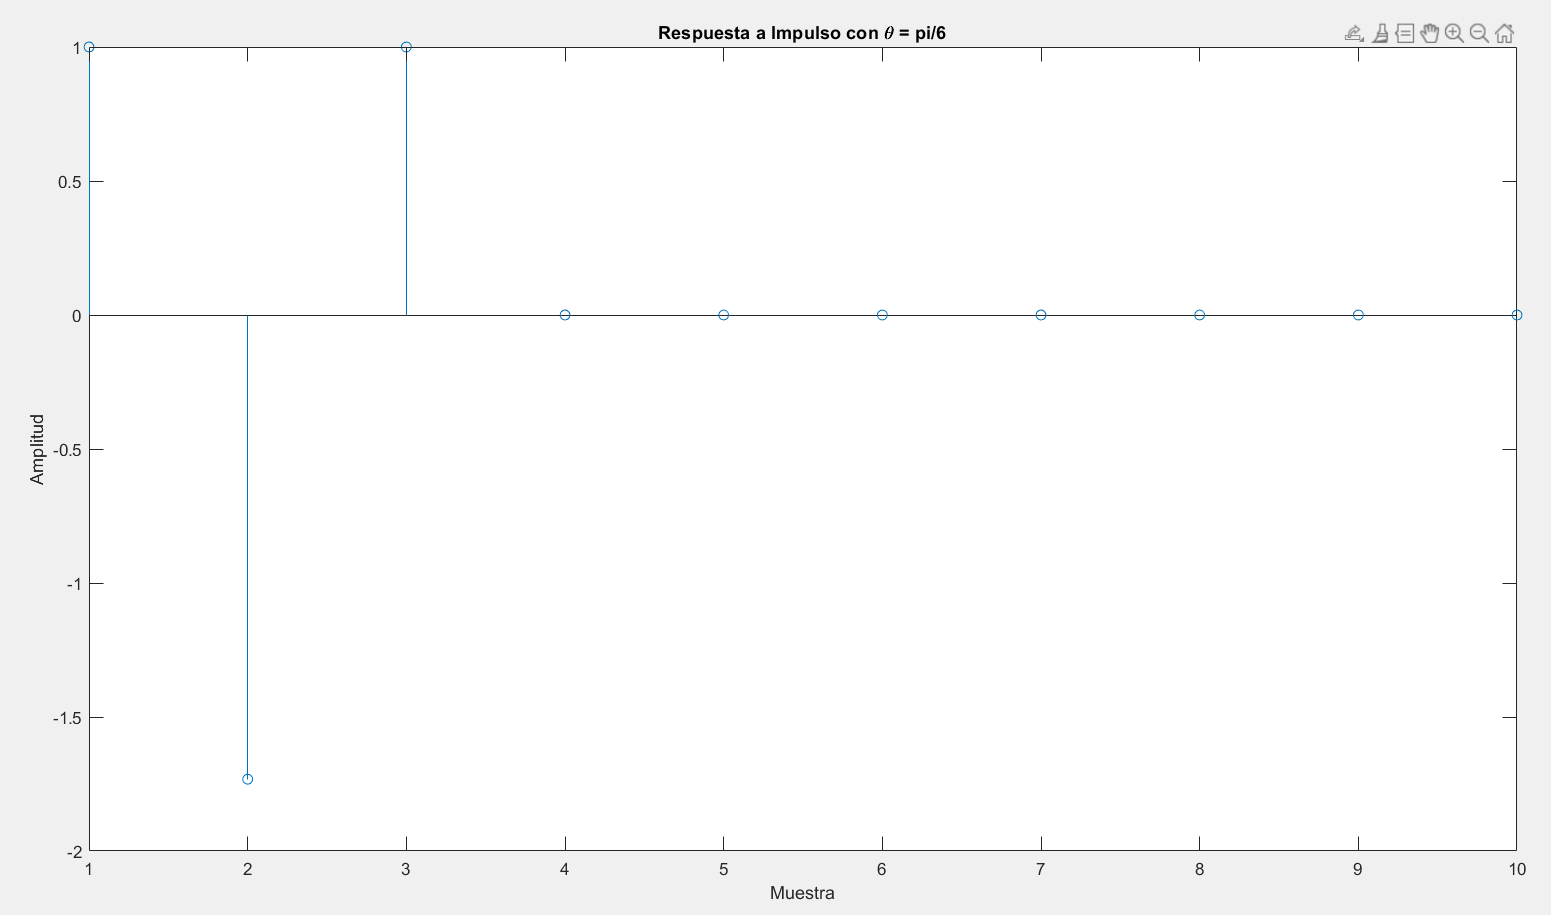
\includegraphics[width=0.75 \linewidth]{Figuras/I_1)_RespuestaImpulso.png}
        \caption{Respuesta impulso con $\theta$ = $\pi /6$.}
        \label{fig:I1}
    \end{figure}
    Donde los coeficientes del filtro $[1~-2Cos( \theta )~1]$ coinciden con las magnitudes.\\ 
    Notamos que se tiene tres muestras distintas de cero para $\theta \neq \frac{\pi (2n - 1) }{2} ~ \forall n = 1, 2, ..$, para los casos en que $Cos( \theta )  = 0 $ se tienen 2 muestras distintas de cero, es decir, el sistema tiene una respuesta impulso finita. \\[0.5 cm]
    
    Para la expresión analítica tenemos en función de $\omega$ tenemos:
    
    \begin{equation*}
    \begin{split}
        H(z) &= 1 - 2 z^ {-1}  Cos (\theta) + z^{-2} \\
        \Rightarrow H( \omega ) &= H (z = e^{j \omega } ) =  \frac{e^{j2 \omega } - 2 e^{j \omega} 
        Cos( \theta ) + 1 }{ e ^{j2 \omega }}\\
    \end{split}
    \end{equation*}
    Cuyo gráfico se muestra a continuación
    \begin{figure}[H]
        \centering
        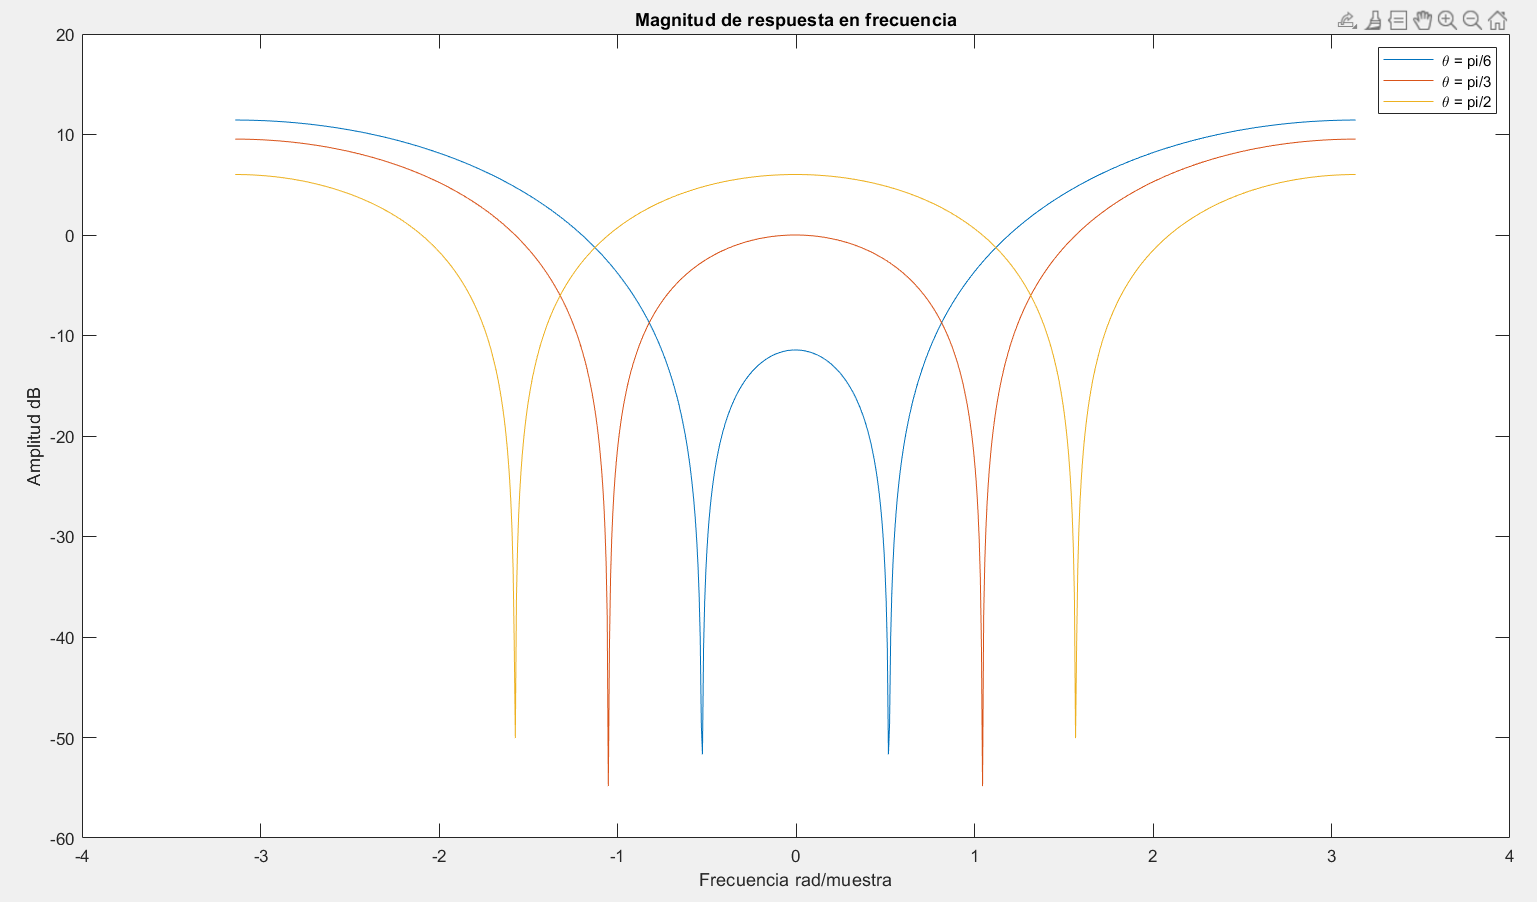
\includegraphics[width=0.75 \linewidth]{Figuras/I_1)_MagH(w).png}
        \caption{Magnitud Respuesta impulso para diferentes valores $\theta $.}
        \label{fig:I1_2}
    \end{figure}
    Podemos notar de la Figura \ref{fig:I1_2}, que la magnitud es disminuida donde $ \omega = \theta $. Esto ocurre porque los ceros del filtros están ubicados en la frecuencia $\theta$, por lo que la respuesta en frecuencia del filtro se anula en esos puntos. $\omega$ corresponde a la frecuencia normalizada en $rad/muestra$, la cual está dada por la relación $\omega = 2*pi*(f_0/f_s)$. Donde $f_0~Hz$ es la frecuencia filtrada.
    
    
    
    
    \item %2)-------------------------------------------------------------------------%
    
    Obtenemos la ecuación de diferencias del filtro descrito considerando un sistema causal como se muestra a continuación.
    \begin{equation*}
    \begin{split}
        H(z) &= \frac{z^2(1-r)}{(z - re^{j \theta})(z - re^{-j \theta})} \\
        &= \frac{z^2(1-r)}{z^2 -zr( e^{j \theta } + e ^{ -j \theta }) + r^2} \\
        &= \frac{1-r}{1 -z^{-1}r Cos( \theta)  + r^2z^{-2}}  \{ \cdot \}  \\
        \Rightarrow y[n] &=  (1-r)x[n] +2ry[n-1]Cos(\theta)-r^2y[n-2] \\
    \end{split}
    \end{equation*}
    
    La gráfica de la respuesta a impulso se muestra en la Figura \ref{fig:I2} para un ángulo $\theta = \pi/6 $ y $r = 0.3$. \\
    Obtenemos la función analítica en función de $\omega $ de la siguiente manera:
    \begin{equation*}
    \begin{split}
        H(z) &=\frac{z^2(1-r)}{z^2 -zrCos(\theta ) + r^2}\\
        \Rightarrow H( \omega ) &= H (z = e^{j \omega } ) = \frac{e^{j2 \omega }(1-r)}{e^{j2 \omega } -e^{j \omega }rCos( \theta ) + r^2}\\
    \end{split}
    \end{equation*}
    El gráfico de la respuesta en frecuencia para diferentes valores de $r$ con $\theta = \pi /3$ se presenta en la Figura \ref{fig:I2_2} donde podemos ver los efectos de $r$, notamos que al aumentarlo, la frecuencia de paso se acerca al valor deseado de $\theta_0$. Esto ocurre porque los polos están ubicados dentro del circulo unitario, pero la respuesta en frecuencia es evaluada sobre el circulo unitario. 
    
    Al aumentar $r$, al evaluar la respuesta en frecuencia en $e^{j\theta_0}$, el valor del polo $e^{j\theta_0}-re^{j\theta_0}$, se va acercando a $0$, por lo que la ganancia aumenta.
    
    \begin{figure}[H]
        \centering
        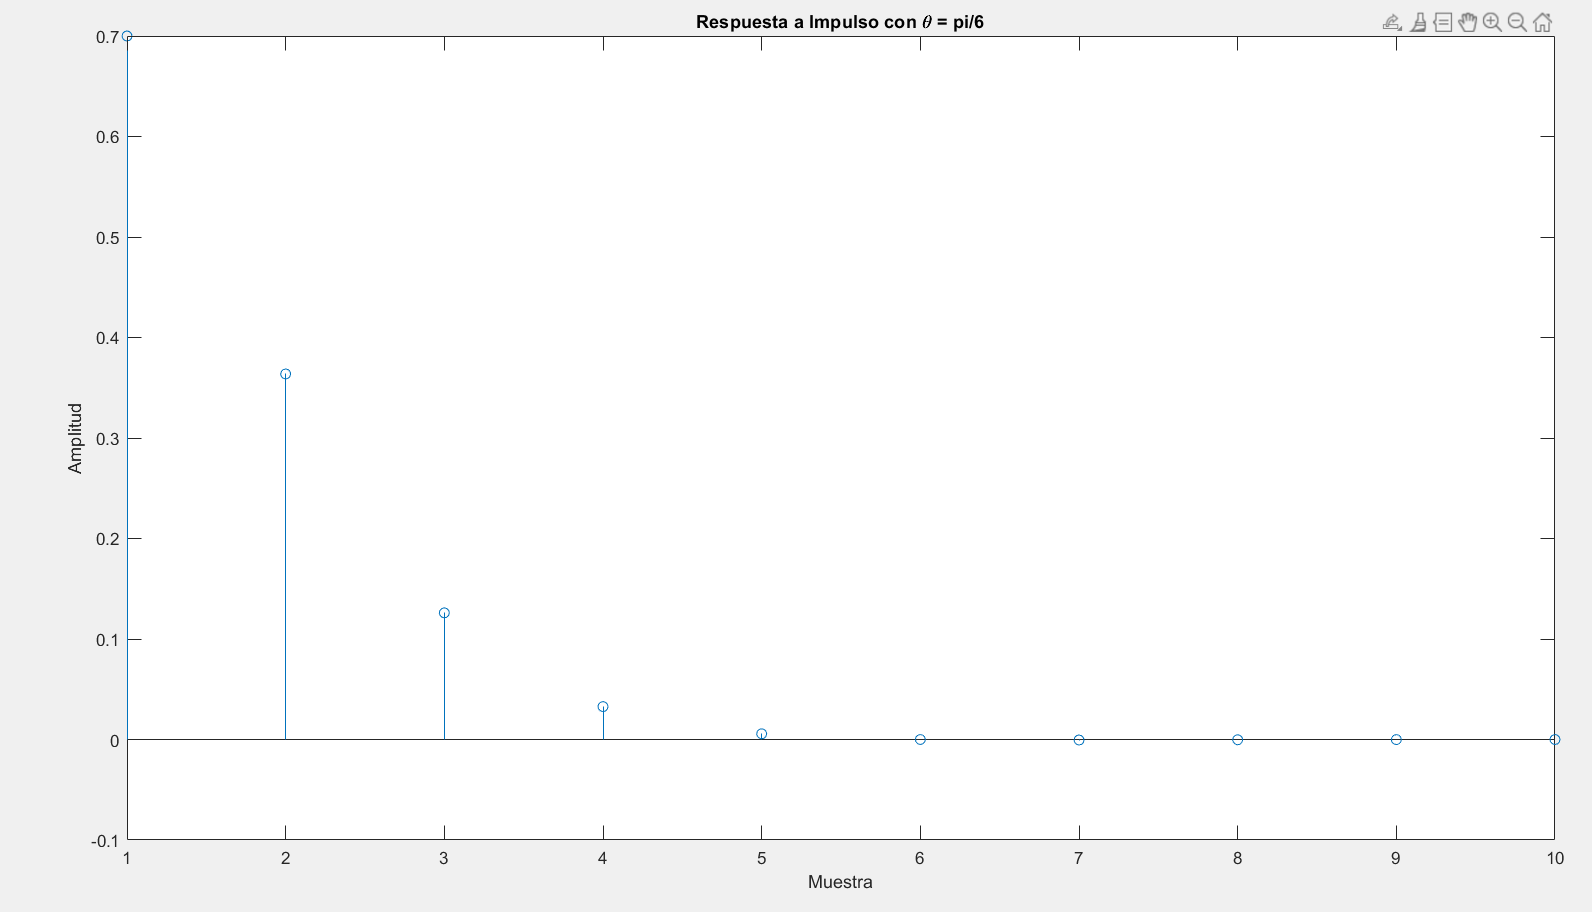
\includegraphics[width=0.75 \linewidth]{Figuras/I_2)_RespuestaImpulso.png}
        \caption{Respuesta impulso con $\theta$ = $\pi /6$ y $r = 0.3$.}
        \label{fig:I2}
    \end{figure}
    \begin{figure}[H]
        \centering
        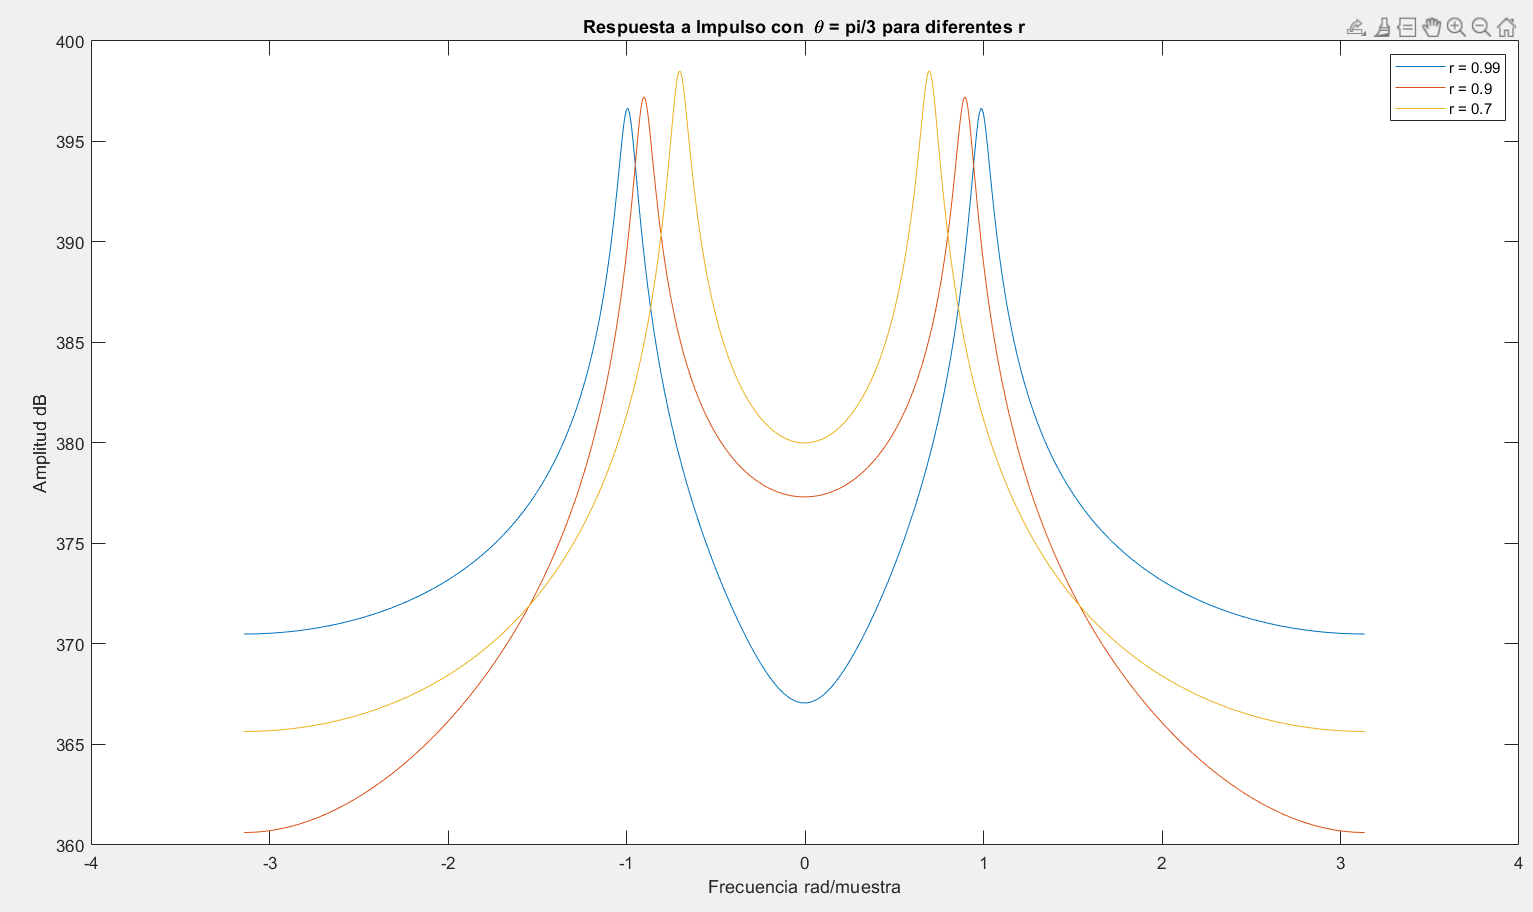
\includegraphics[width=0.75 \linewidth]{Figuras/I_2)_MagH(w).png}
        \caption{Magnitud Respuesta impulso para diferentes valores de $r$.}
        \label{fig:I2_2}
    \end{figure}
    
    \item %3)-------------------------------------------------------------------------%
    Para implementar el filtro FIR utilizamos el siguiente código:
    \begin{lstlisting}
    function y = FIR_filter(x,theta)
    b = [1 -2*cos(theta) 1];
    a = [1 0 0];
    h = impz(b,a);
    y = conv(h,x);
    end
    \end{lstlisting}
    
    Aplicamos el comando $plot\_fft\_mag$ a la señal $nspeech$ lo que se muestra en la Figura \ref{fig:I3_FFT} donde rescatamos el tono a filtrar $frec = 1685 ~Hz$
    \begin{figure}[H]
        \centering
        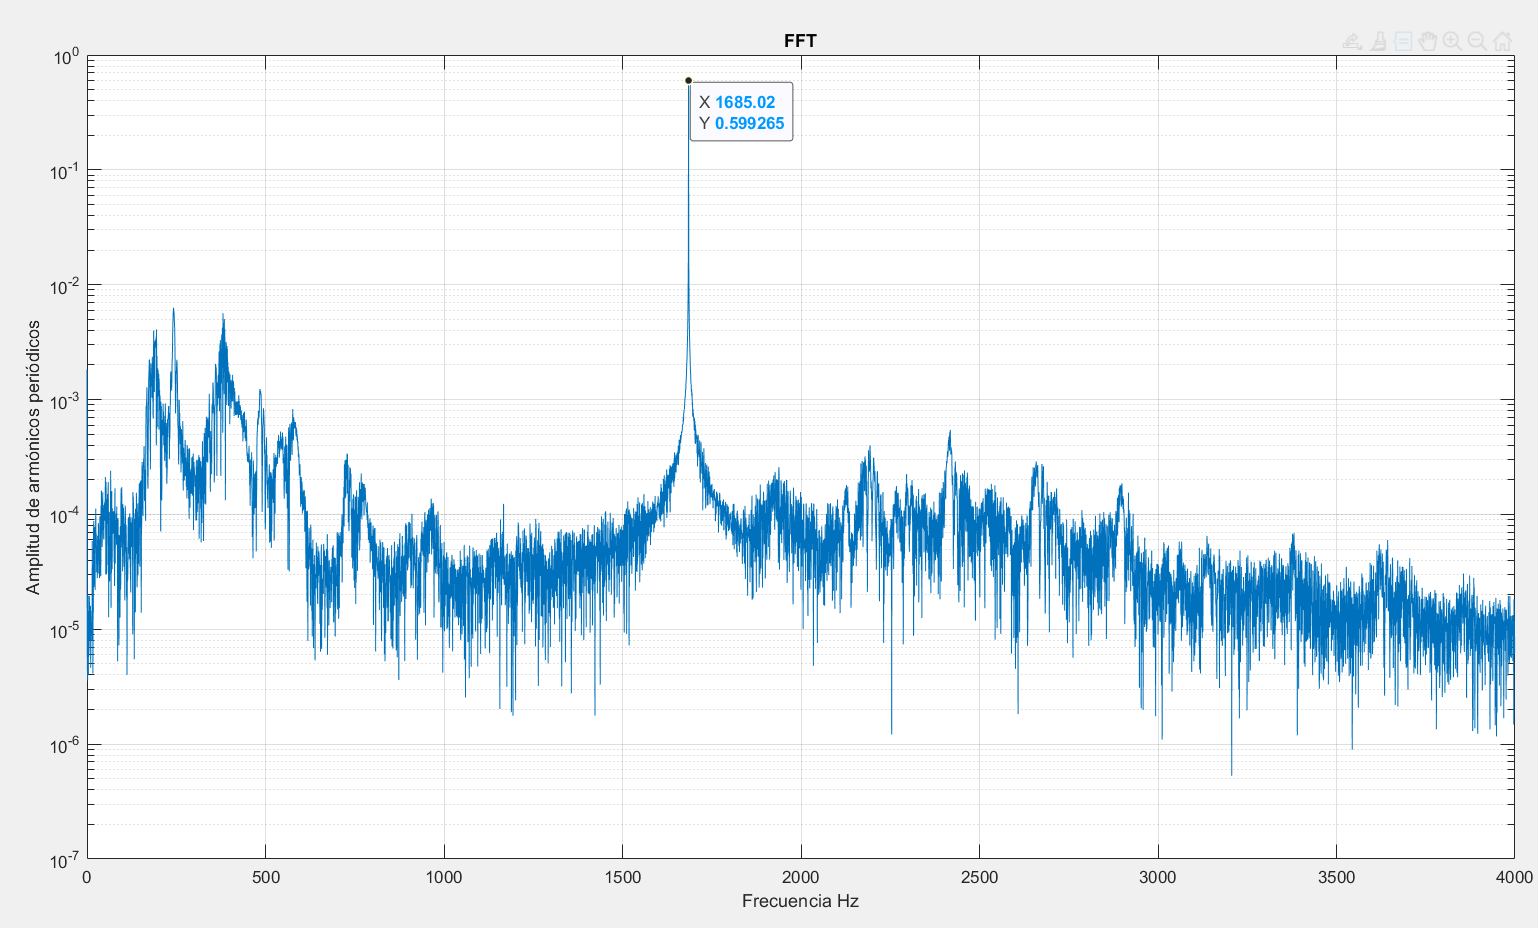
\includegraphics[width=0.75 \linewidth]{Figuras/I_3)_FFT.png}
        \caption{FFT de nspeech.}
        \label{fig:I3_FFT}
    \end{figure}

    tenemos que la frecuencia de muestreo es $f_s = 8000~Hz$ por lo que normalizamos la frecuencia a filtrar de la siguiente manera:
    \begin{equation*}
        f_n = \frac{frec \cdot 2 \pi}{f_s} = \frac{1685 \cdot 2 \pi }{ 8000 } = 1.3234 ~ rad/muestra
    \end{equation*}
    Al aplicar como entrada $nspeech$ junto a $f_n$ al filtro FIR antes descrito, se obtienen los coeficientes $b_k = [1~-0.4898~1]$. El resultado al aplicar el filtro se observa en la Figura \ref{fig:I3_nspeech}, donde notamos que se filtra perfectamente el tono especificado.
    \begin{figure}[H]
        \centering
        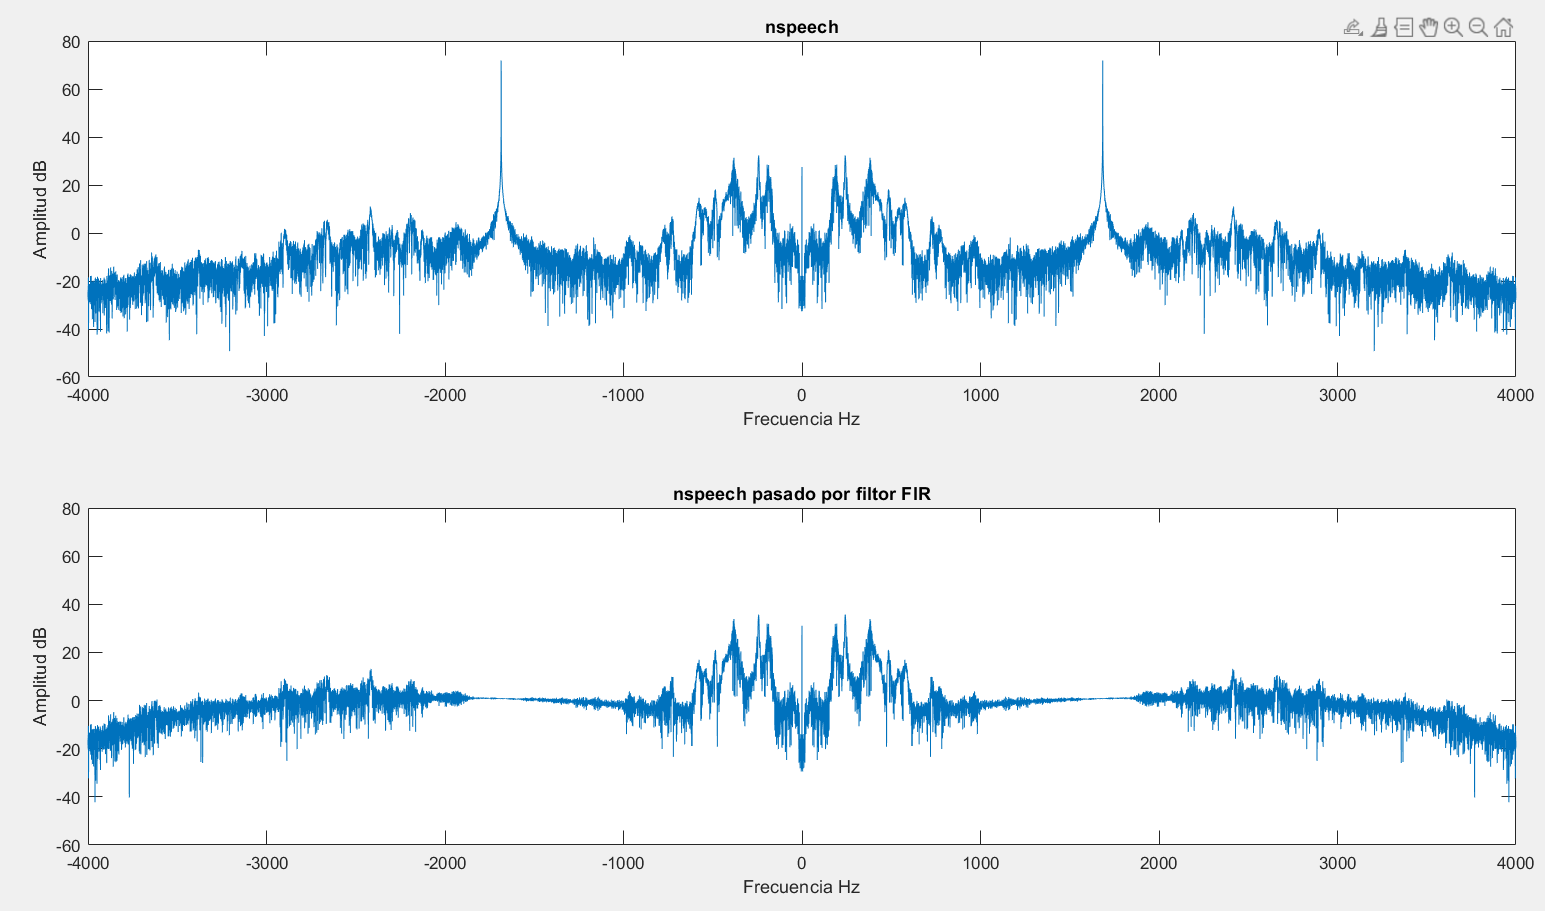
\includegraphics[width=0.75 \linewidth]{Figuras/I_3)_conv.png}
        \caption{Filtrado usando Convolución.}
        \label{fig:I3_nspeech}
    \end{figure}
    Comparando el filtro FIR implementado anteriormente con el filtro de $Matlab$ implementado de la siguiente manera:
    \begin{lstlisting}
    senal_filtrada2 = filter([1 -2*cos(fn) 1],[1 0 0], nspeech);
    \end{lstlisting}
    Obtenemos el resultado mostrado en la Figura \ref{fig:I3_nspeech2}. En ambos casos se logra eliminar el tono esperado.\\ Notamos que el largo del resultado de filtro por convolución es más largo debido a que al operar la convolución el largo sera la suma de el largo de las señales convolucionadas menos uno. 
    
    \begin{figure}[H]
        \centering
        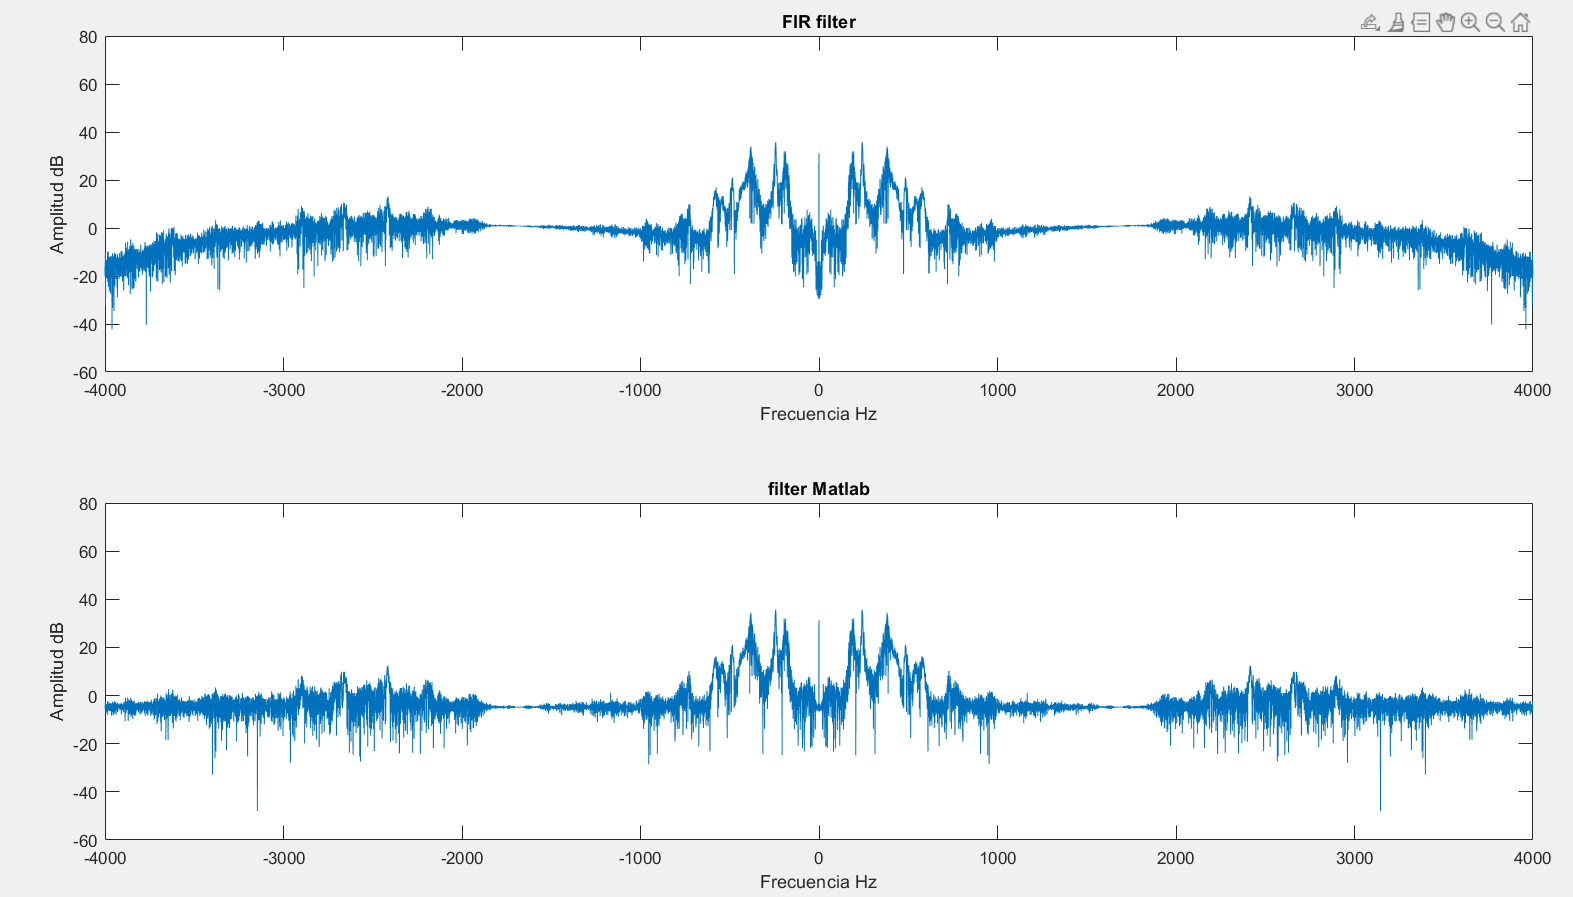
\includegraphics[width=0.75 \linewidth]{Figuras/I_3)_FIRvsFilter.png}
        \caption{FIR filter vs filter Matlab.}
        \label{fig:I3_nspeech2}
    \end{figure}
    \item %4)-------------------------------------------------------------------------%
    Implementamos el filtro IIR con el siguiente código:
    \begin{lstlisting}
    function y = IIR_filter(yBuff, aCoeff, x)
    y_new = x - aCoeff(1)*yBuff(1) - aCoeff(2)*yBuff(2);
    y = [y_new yBuff(1)];
    end
    \end{lstlisting}
    
    Graficamos la FFT de la señal $pcm$, que se muestra en la Figura \ref{fig:I4_FFT}, donde obtenemos la frecuencia deseada del pasa-banda, la cual corresponde $frec = 3146 ~ Hz$, frecuencia que normalizamos para aplicar al filtro quedando $f_n = \frac{frec \cdot 2 \pi}{f_s} = \frac{3156 \cdot 2 \pi }{ 8000 } = 2.4709 ~ rad/muestra$.
    \begin{figure}[H]
        \centering
        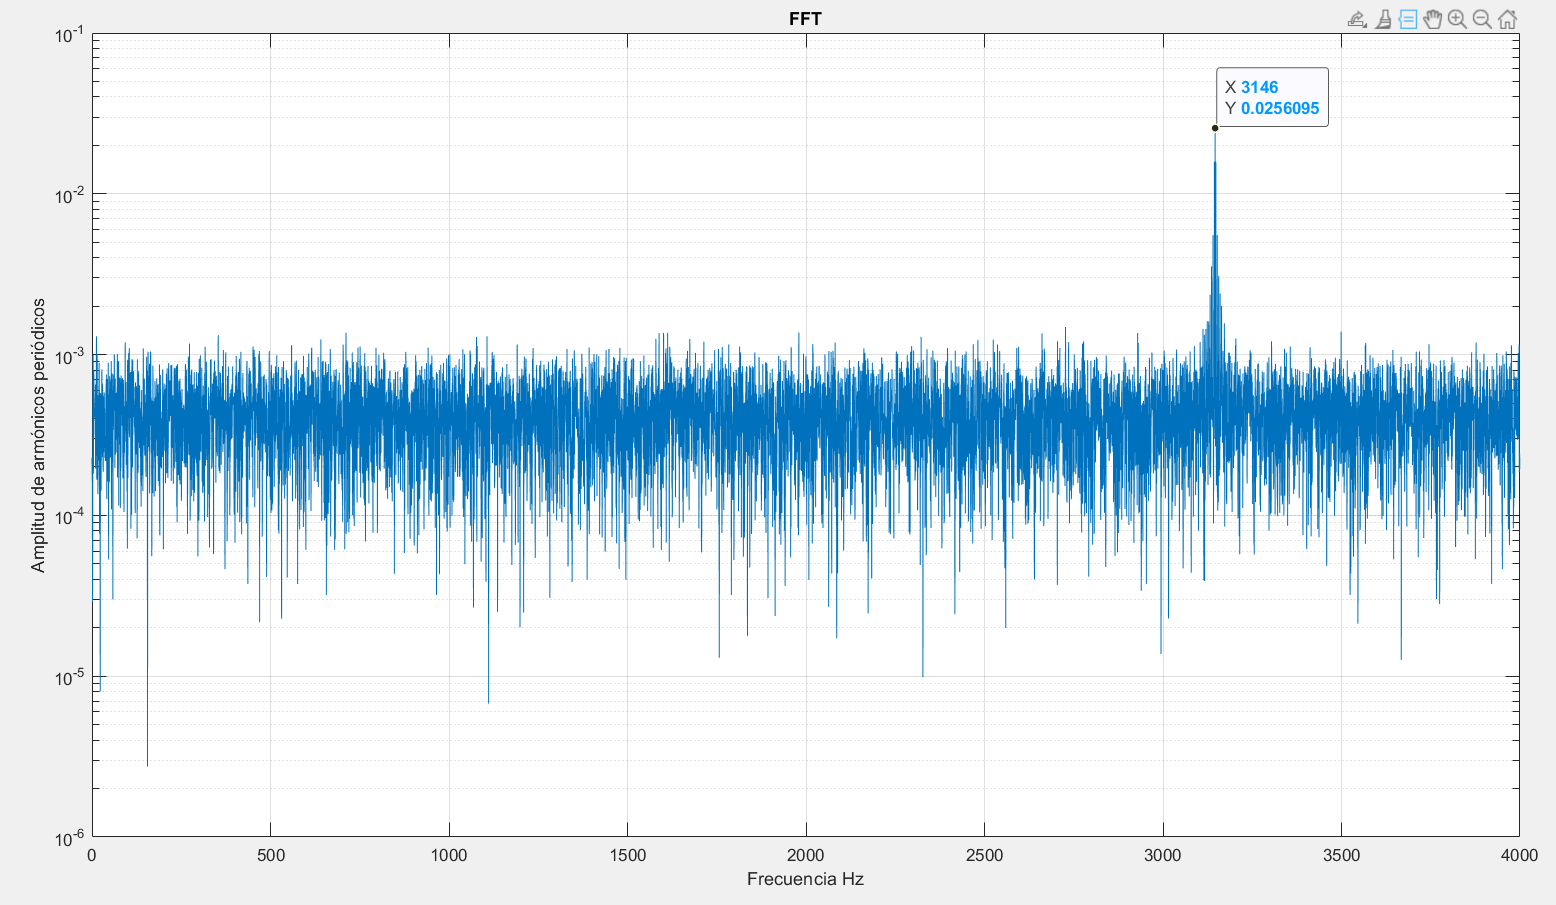
\includegraphics[width=0.75 \linewidth]{Figuras/I_4)_FFT.png}
        \caption{FFT de señal pcm.}
        \label{fig:I4_FFT}
    \end{figure}
\end{enumerate}
Los coeficientes del filtro utilizados corresponden a $a_k = [-2Cos( \theta) ~ r^2] = [1.5511 ~ 0.9801]$ Con los cuales obtenemos los resultados presentados en las Figura \ref{fig:I4_Espectro} y \ref{fig:I4_Temporal}, que muestran la comparación entre la señal $pcm$ original y la respuesta del filtro IIR, en su espectro en frecuencia y en el dominio temporal respectivamente. Notamos que se logra pasar el tono deseado perfectamente, donde en la Figura \ref{fig:I4_Temporal} se aprecia la recuperación de la señal sin ruido.
    \begin{figure}[H]
        \centering
        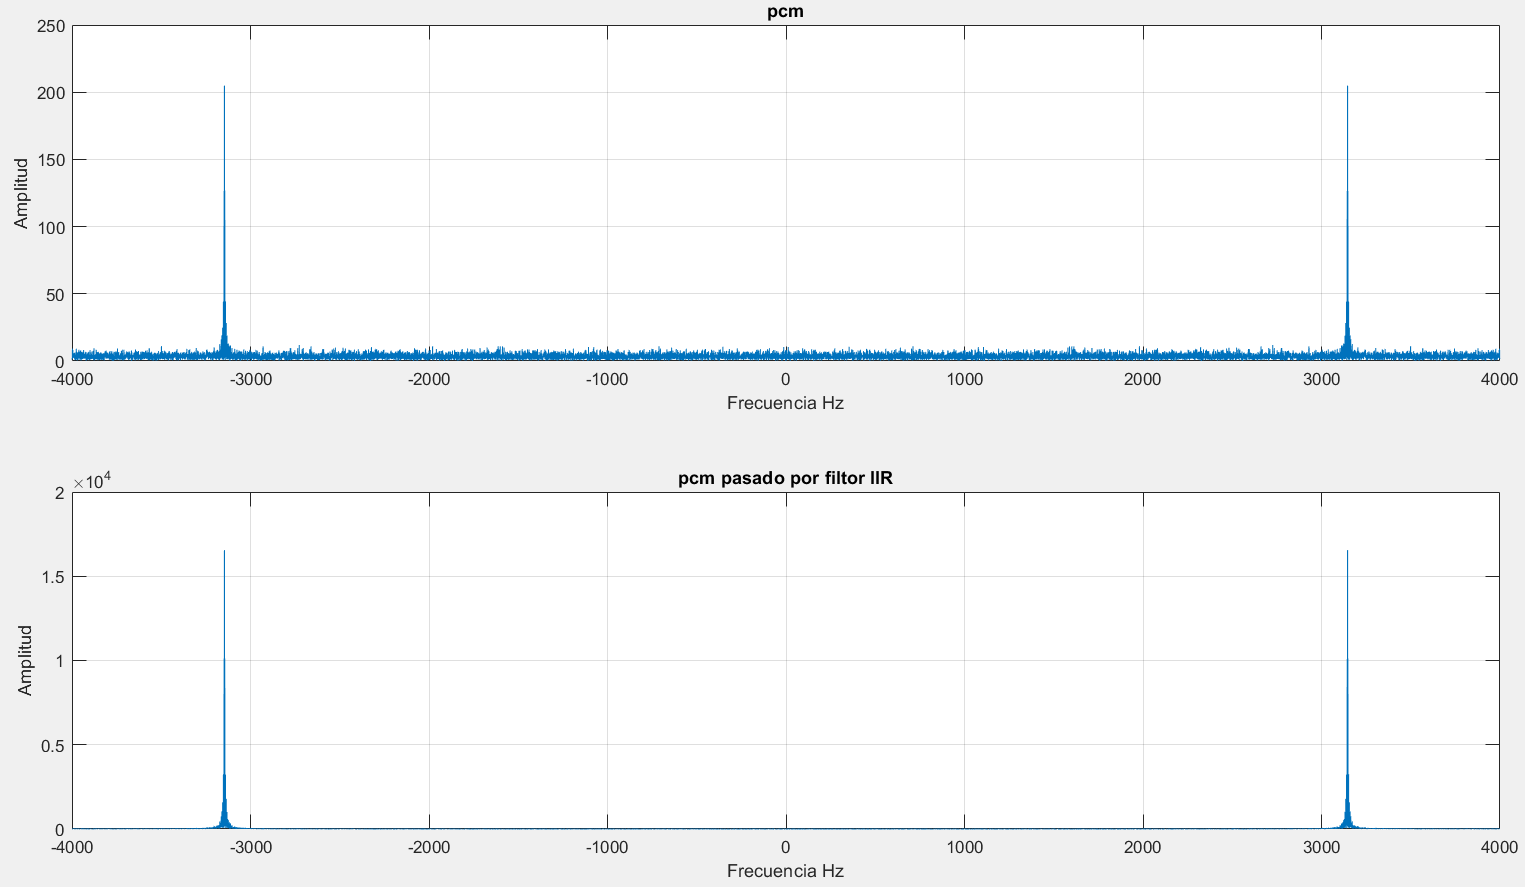
\includegraphics[width=0.75 \linewidth]{Figuras/I_4)_IIR_amplitud.png}
        \caption{Señal pcm vs pcm filtrada, espectro en frecuencia.}
        \label{fig:I4_Espectro}
    \end{figure}
    
    \begin{figure}[H]
        \centering
        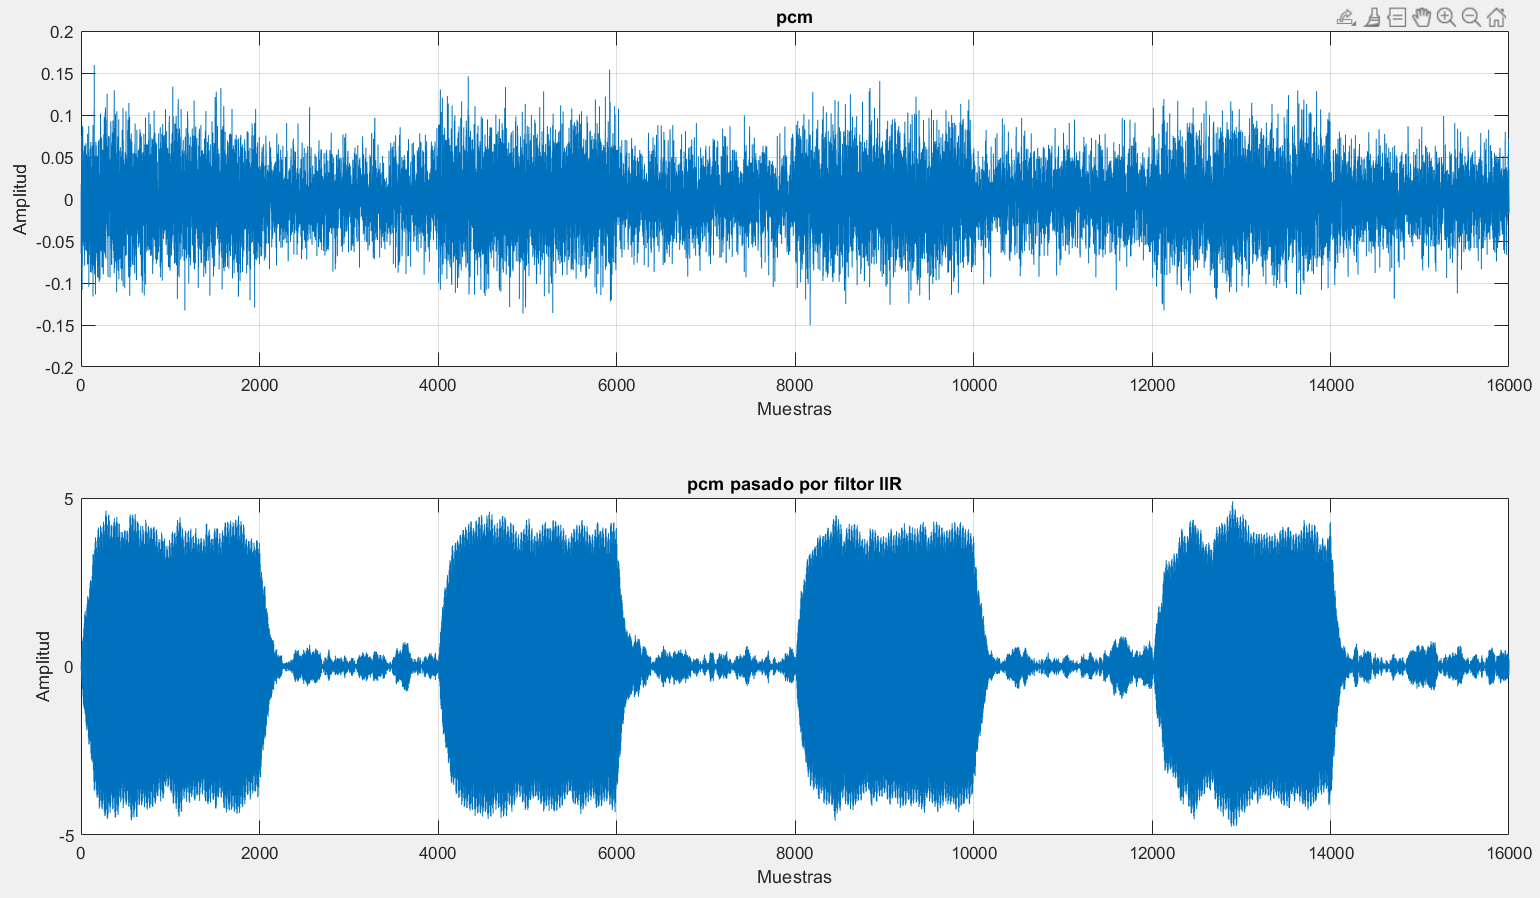
\includegraphics[width=0.75 \linewidth]{Figuras/I_4)_IIR_temproal.png}
        \caption{Señal pcm vs pcm filtrada, dominio temporal.}
        \label{fig:I4_Temporal}
    \end{figure}

%%%%%%%%%%%%%%%%%%%%%%%%%%%%%%%%%%%%%%%%%%%%%%%%%%%%%%%%%%%%%%%%%%%%%%%%%%%%%%%%%
%
%-------------DISE ̃NO DE FILTROSFIRUSANDO VENTANAS----------------------------%
%
%%%%%%%%%%%%%%%%%%%%%%%%%%%%%%%%%%%%%%%%%%%%%%%%%%%%%%%%%%%%%%%%%%%%%%%%%%%%%%%%%
\section{Diseño de filtros FIR usando ventanas}
\begin{enumerate}[1)]
    \item %1)-------------------------------------------------------------------------%
    Obtenemos la magnitud y la fase de los filtros pedidos que se muestran en las Figuras \ref{fig:II_1)N21}, \ref{fig:II_1)N101} y \ref{fig:II_1)N1001} para N iguales a 21, 101, 1001 respectivamente.\\
    De las figuras podemos notar que al aumentar N, la respuesta en magnitud se aproxima más a una ventana rectangular ideal, aumentando su pendiente y aumentando el rechazo de las bandas de rechazo. Notamos en la fase que al aumentar las muestras se asemeja más a una fase lineal, y que su pendiente aumenta.
    \begin{figure}[H]
        \centering
        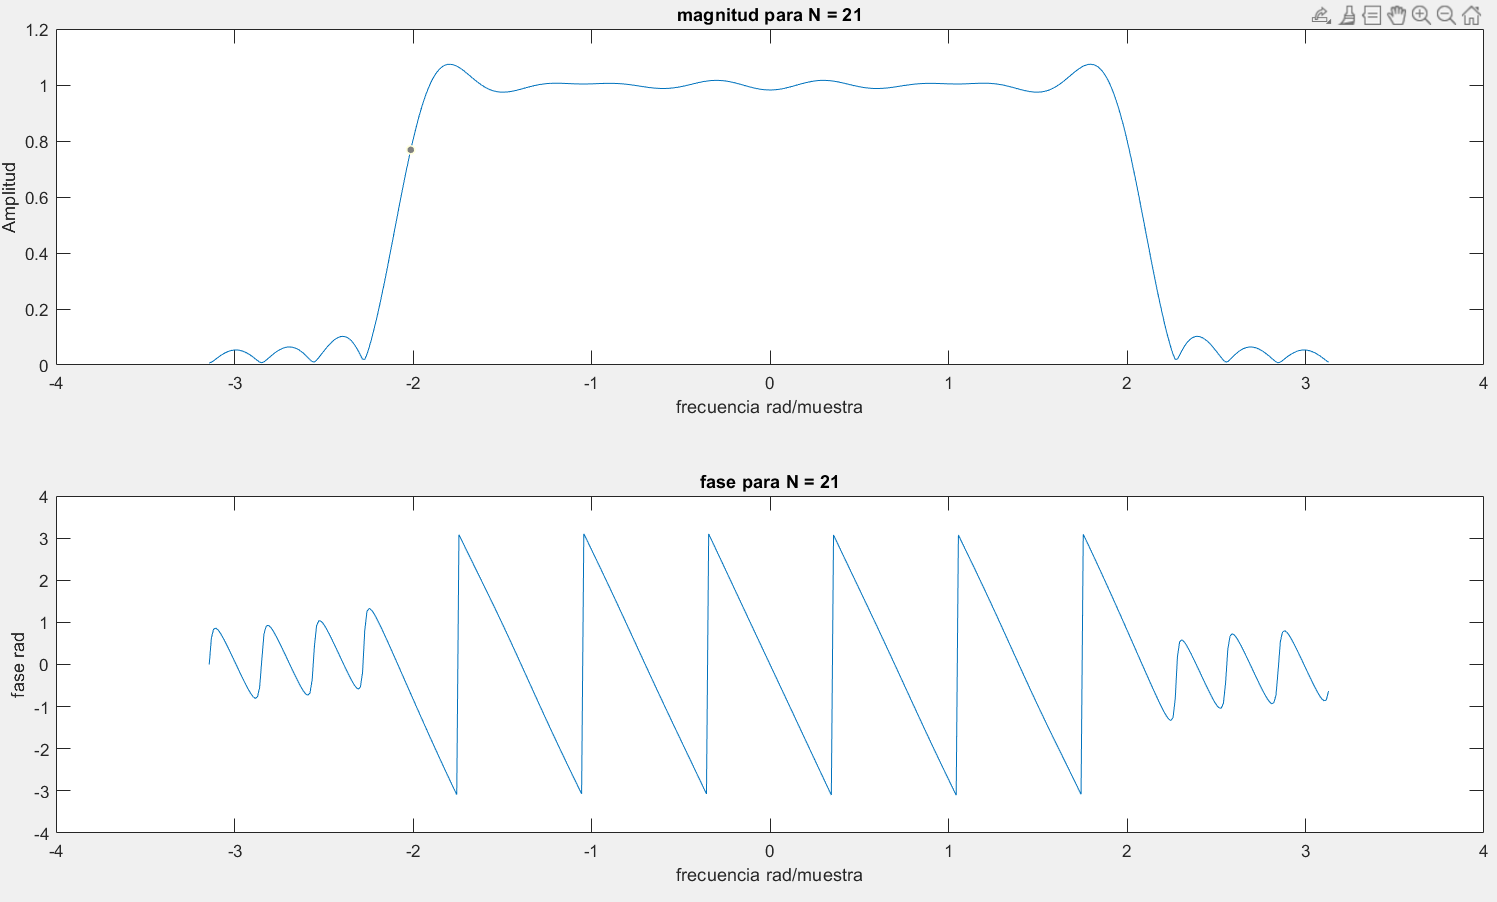
\includegraphics[width=0.75 \linewidth]{Figuras/II_1)N21.png}
        \caption{Amplitud y fase para filtro FIR de ventana con N = 21.}
        \label{fig:II_1)N21}
    \end{figure}
    \begin{figure}[H]
        \centering
        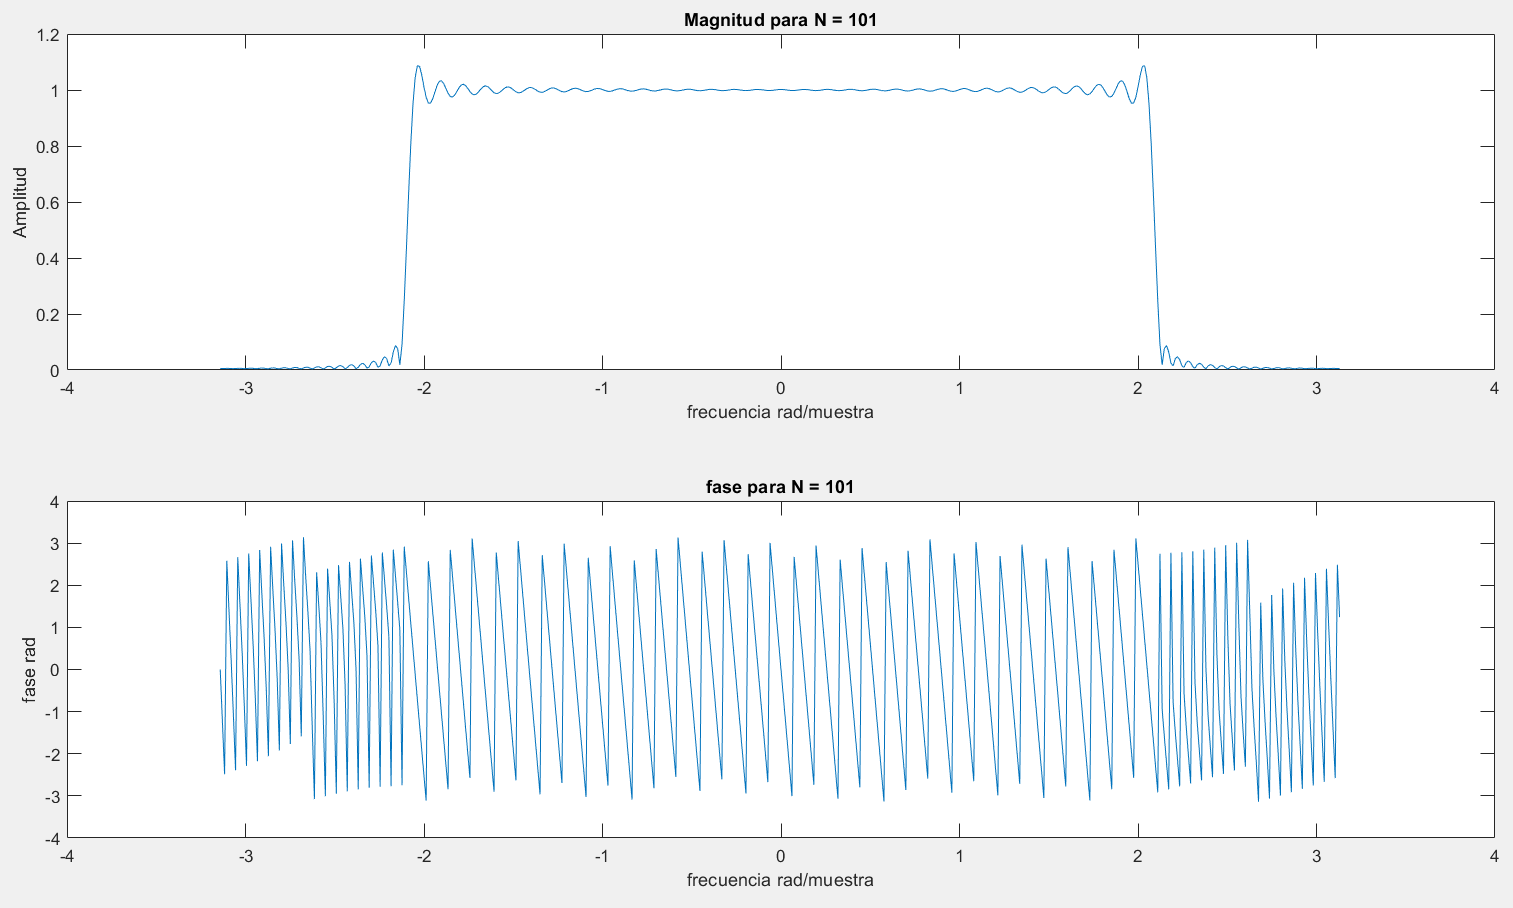
\includegraphics[width=0.75 \linewidth]{Figuras/II_1)N101.png}
        \caption{Amplitud y fase para filtro FIR de ventana con N = 101.}
        \label{fig:II_1)N101}
    \end{figure}
    \begin{figure}[H]
        \centering
        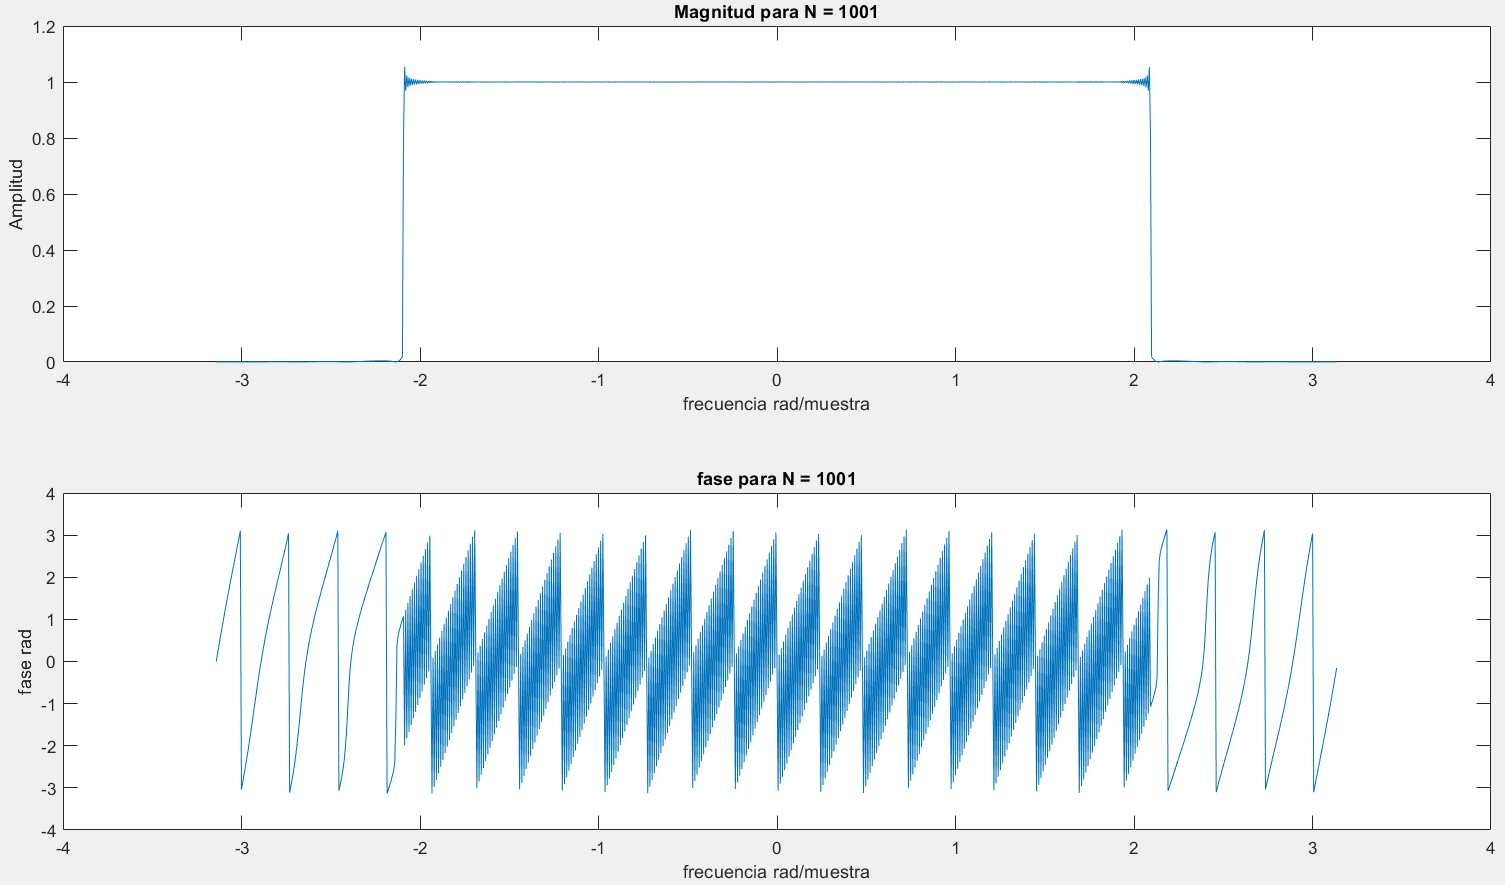
\includegraphics[width=0.75 \linewidth]{Figuras/II_1)N1001.png}
        \caption{Amplitud y fase para filtro FIR de ventana con N = 1001.}
        \label{fig:II_1)N1001}
    \end{figure}
    \item %2)-------------------------------------------------------------------------%
    En la Figura \ref{fig:II_2)ventanas} se muestran las 5 ventanas.
    \begin{figure}[H]
        \centering
        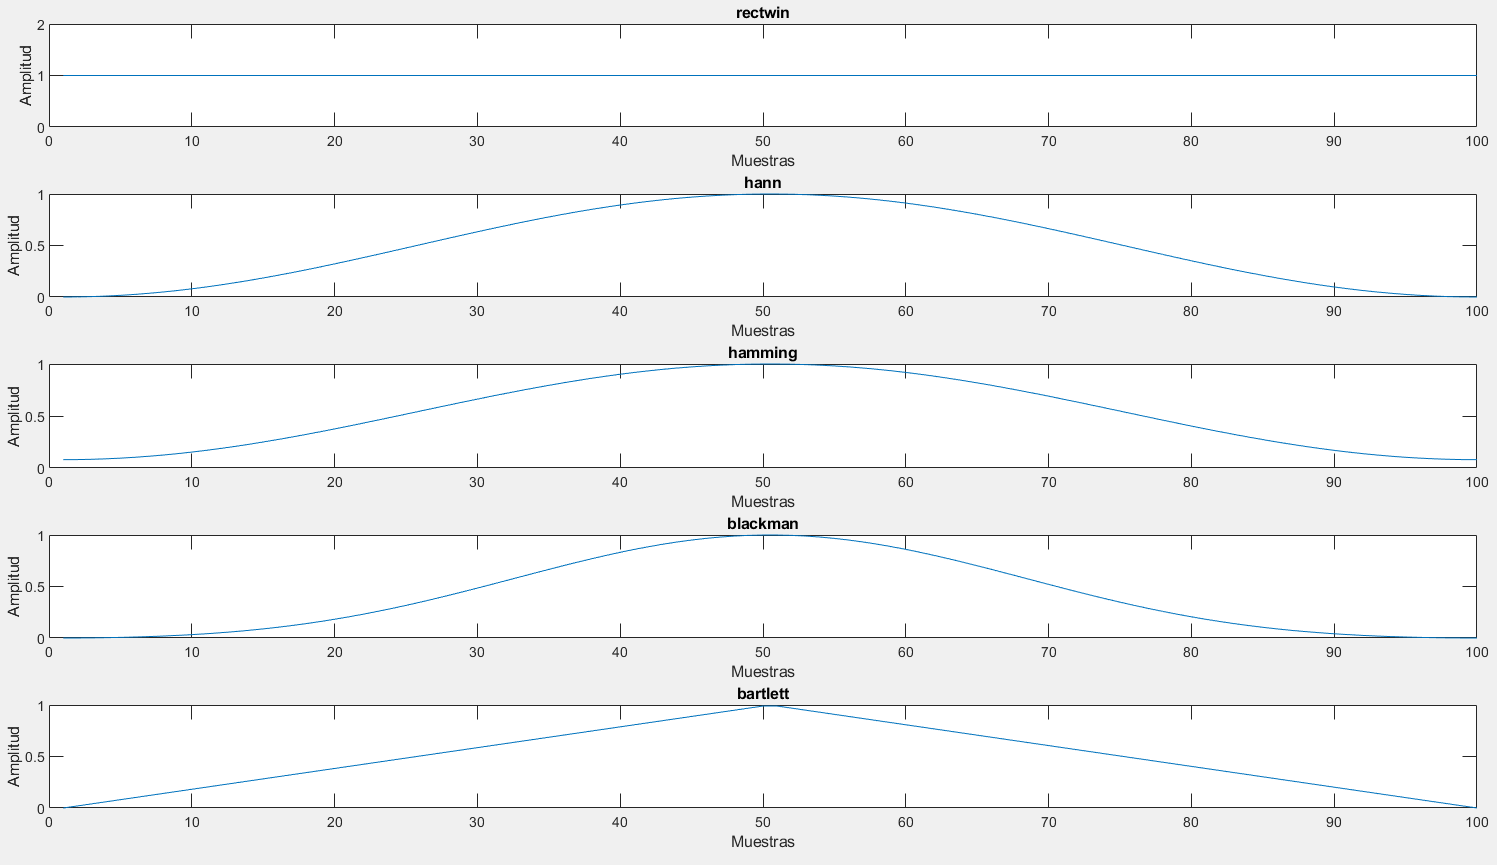
\includegraphics[width=0.75 \linewidth]{Figuras/II_2)Ventanas.png}
        \caption{Ventanas generadas.}
        \label{fig:II_2)ventanas}
    \end{figure}
    A continuación se presenta la magnitud y la fase del espectro de cada una de las ventanas.
    \begin{figure}[H]
        \centering
        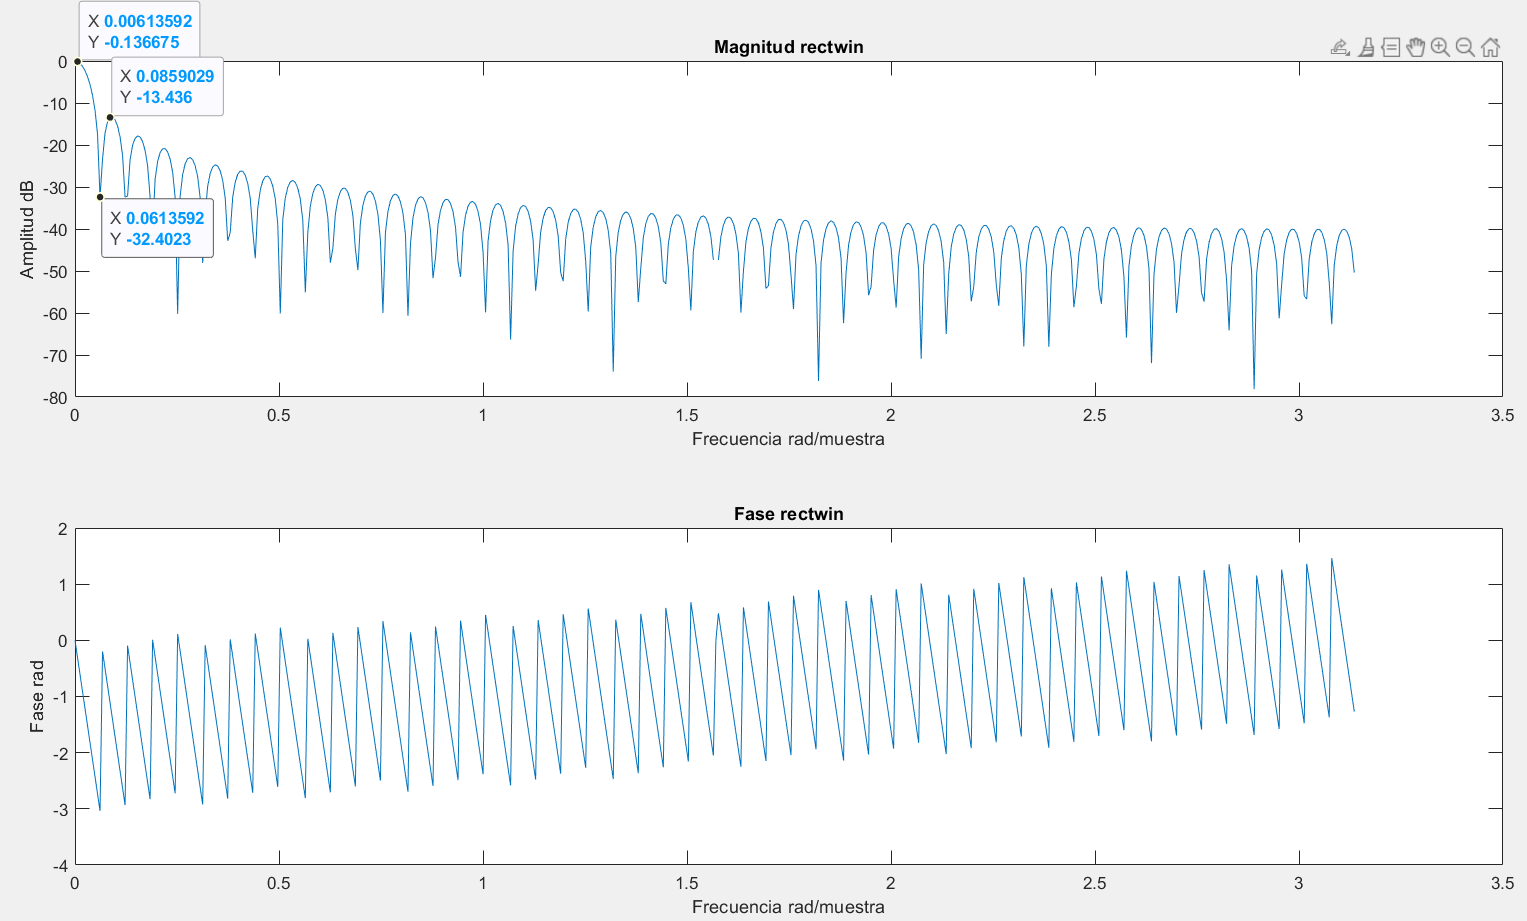
\includegraphics[width=0.75 \linewidth]{Figuras/II_2)rectwin_dB.png}
        \caption{Ventana rectangular.}
        \label{fig:II_2)rect}
    \end{figure}
    \begin{figure}[H]
        \centering
        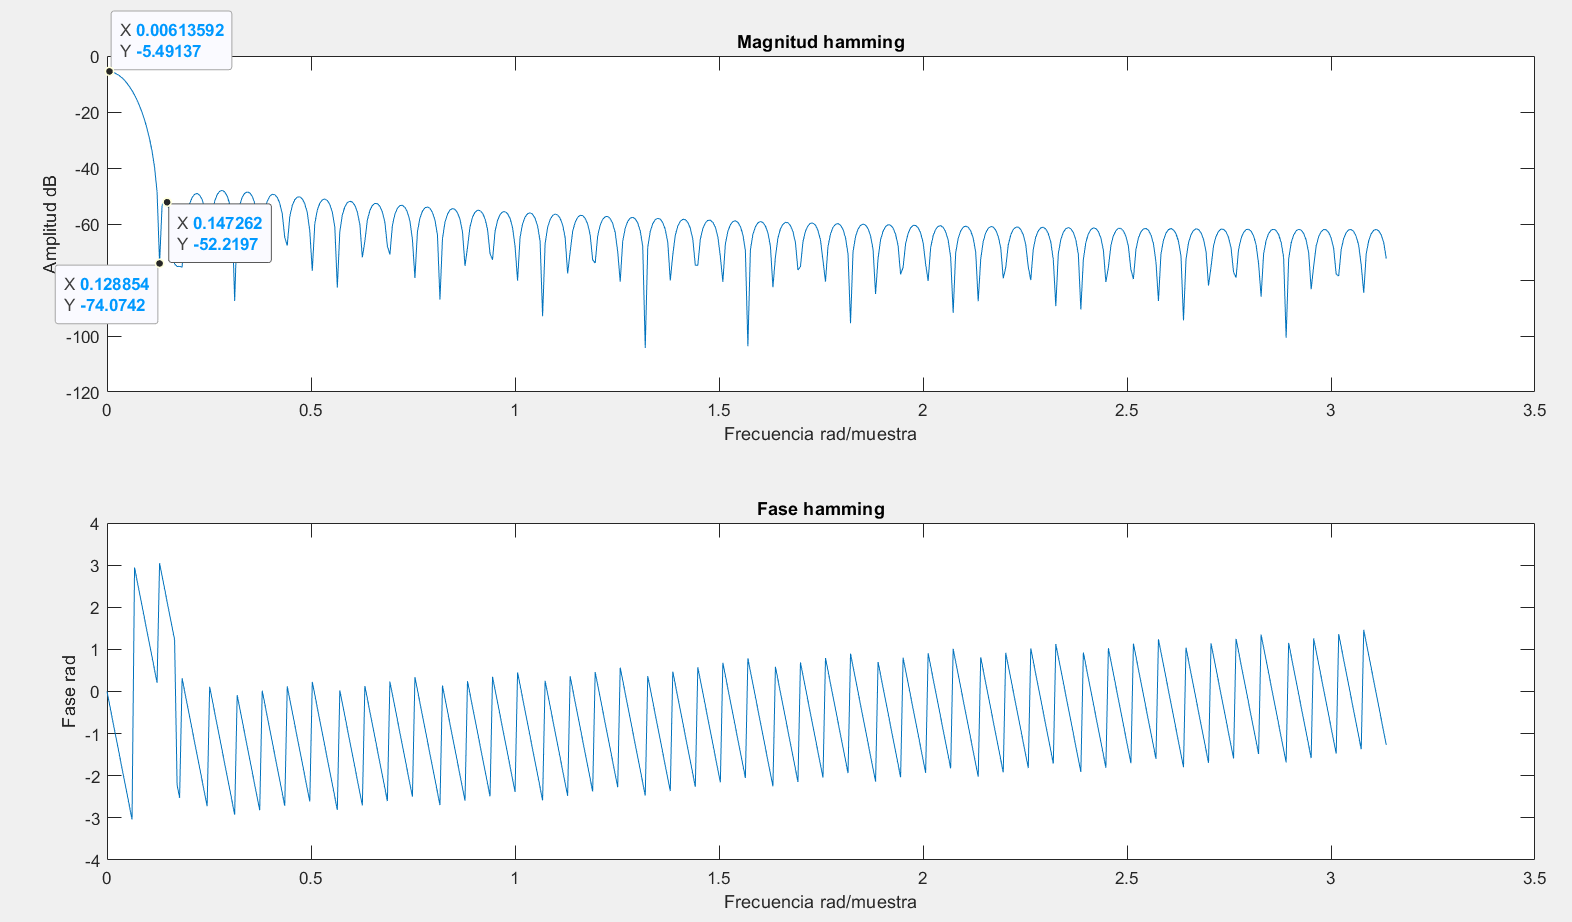
\includegraphics[width=0.75 \linewidth]{Figuras/II_2)hamming_dB.png}
        \caption{Ventana hamming.}
        \label{fig:II_2)ham}
    \end{figure}
    \begin{figure}[H]
        \centering
        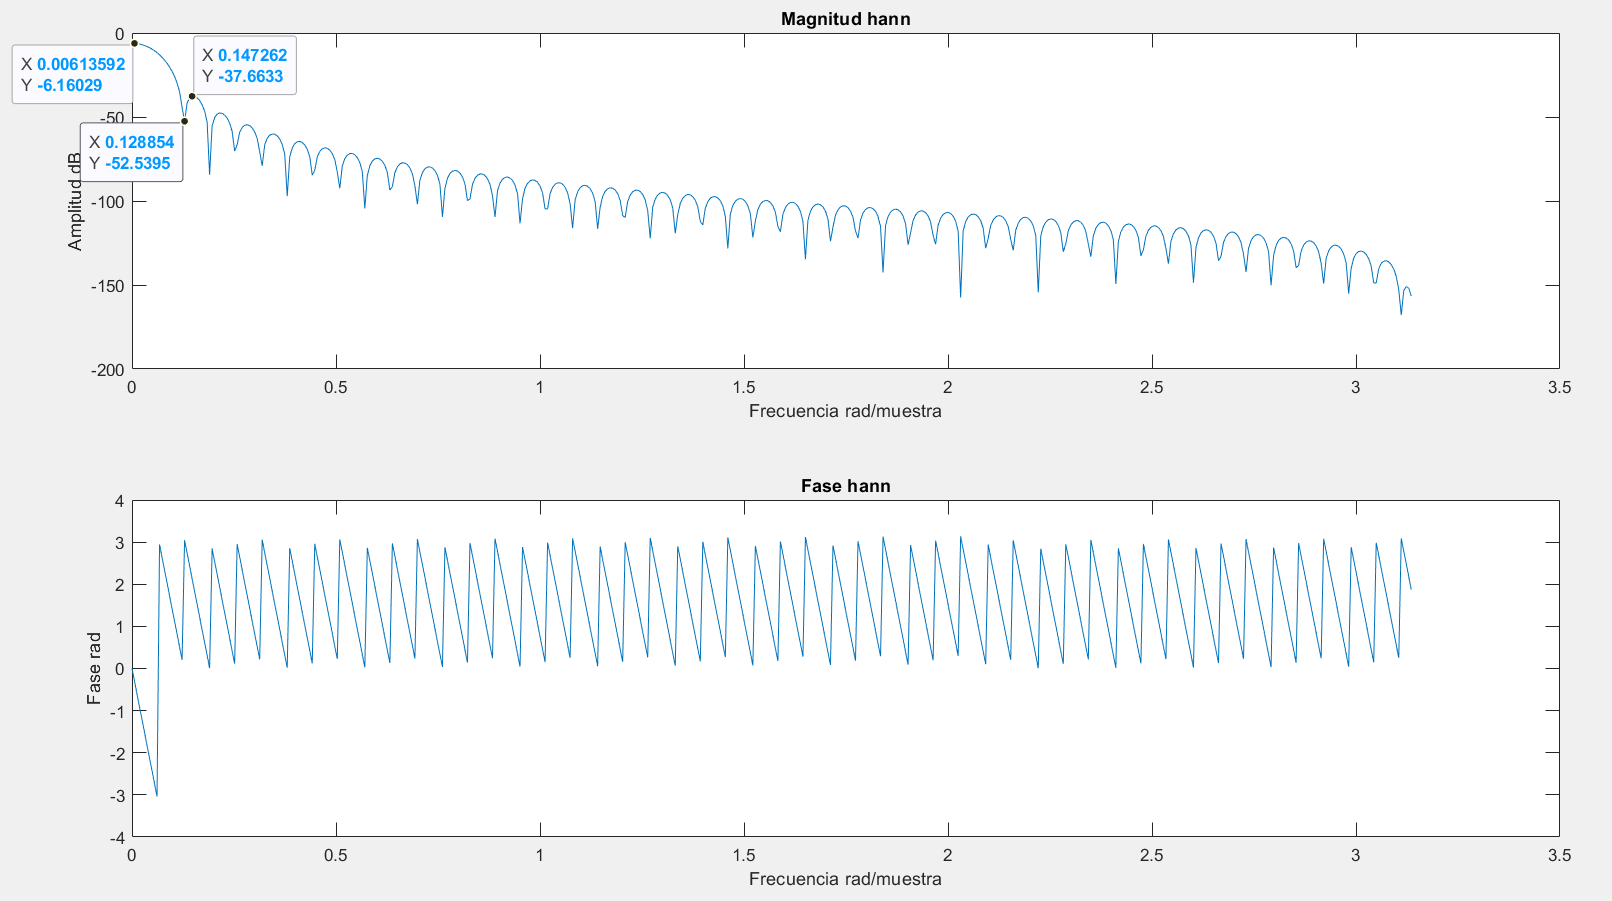
\includegraphics[width=0.75 \linewidth]{Figuras/II_2)hann_dB.png}
        \caption{Ventana hanning.}
        \label{fig:II_2)han}
    \end{figure}
    \begin{figure}[H]
        \centering
        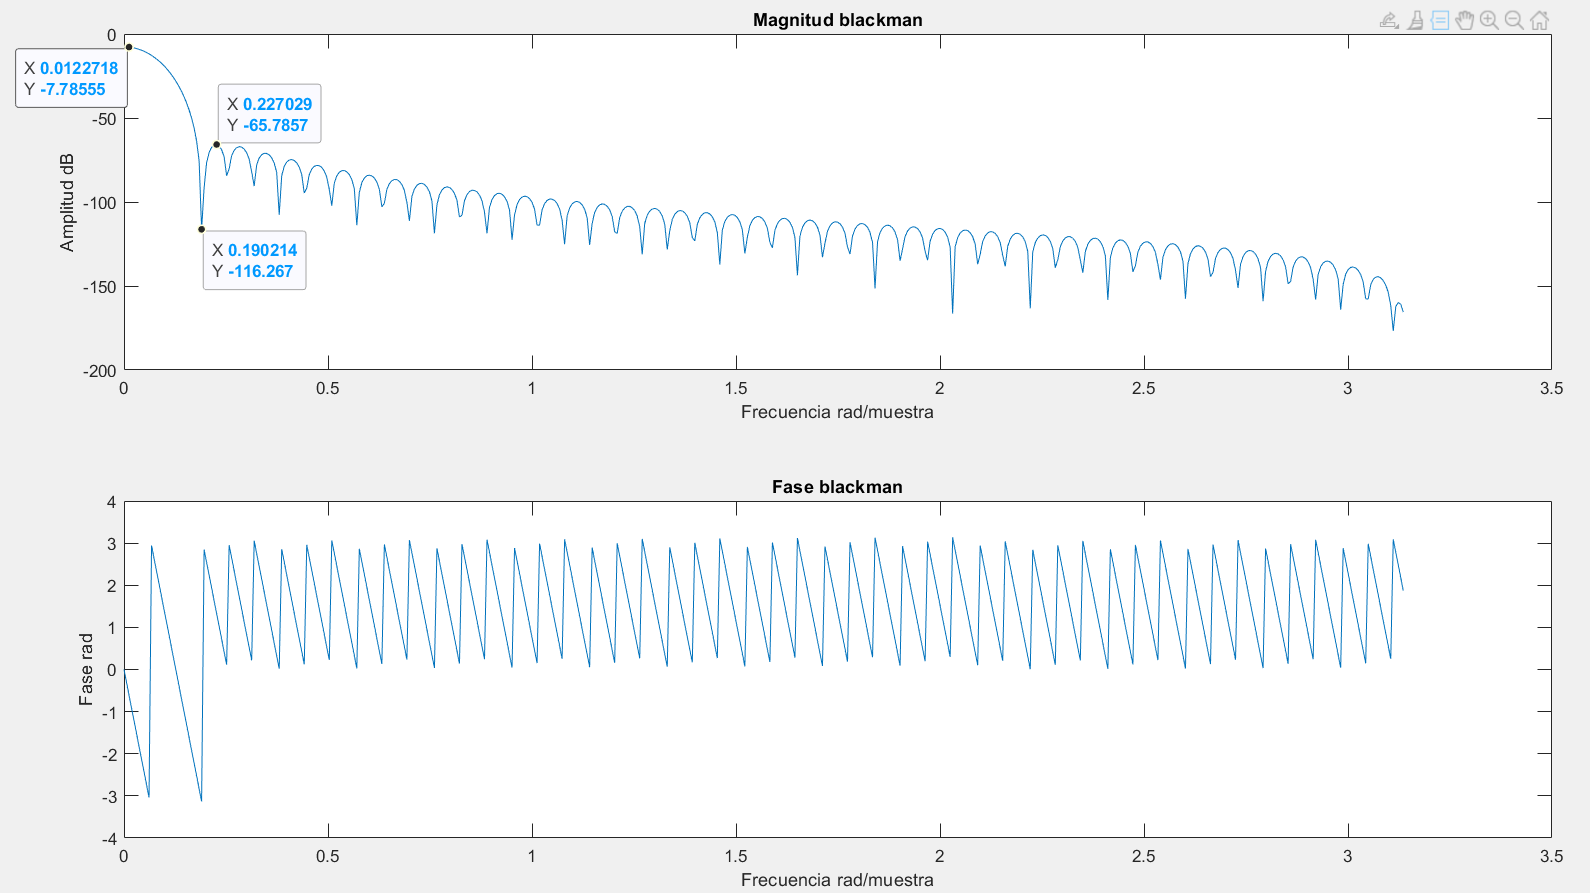
\includegraphics[width=0.75 \linewidth]{Figuras/II_2)blackman_dB.png}
        \caption{Ventana blackman.}
        \label{fig:II_2)blackman}
    \end{figure}
    \begin{figure}[H]
        \centering
        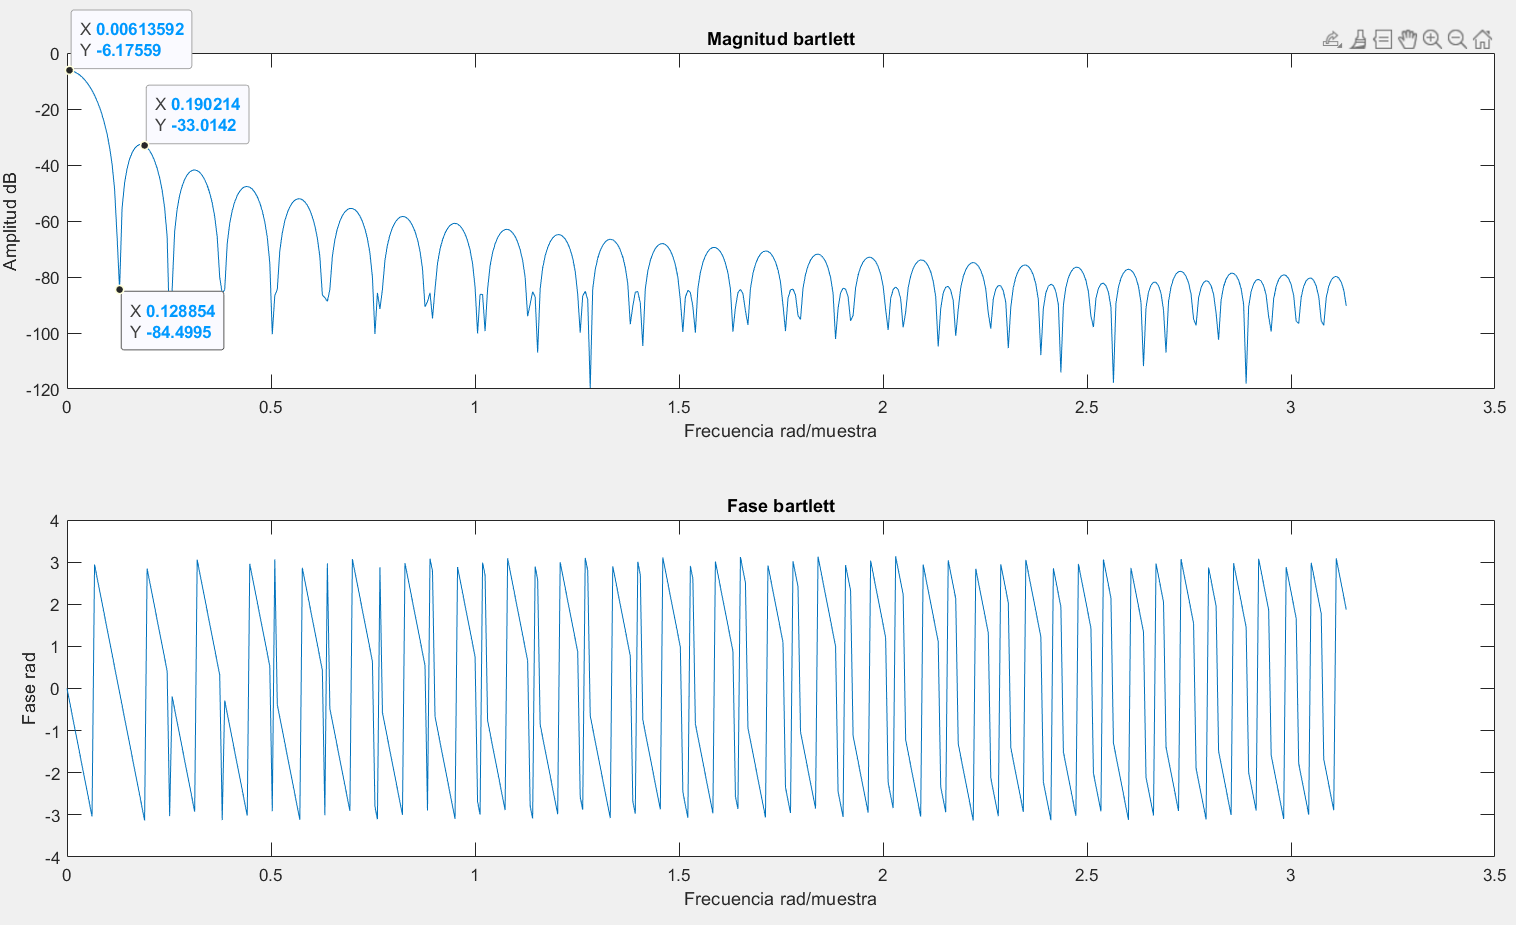
\includegraphics[width=0.75 \linewidth]{Figuras/II_2)barlett_dB.png}
        \caption{Ventana bartlett.}
        \label{fig:II_2)barlett}
    \end{figure}
\end{enumerate}
La tabla de comparación se muestra a continuación
\begin{table}[H]
        \centering
        \begin{tabular}{|c|c|c|}
        \hline
            Ventana     & Ancho de Mainlobe rad/muestra & Amplitud relativa a sidelobe dB \\ \hline
            Rectangular & 0.061 & 13 \\
            Hamming     & 0.128 & 46 \\
            Hanning     & 0.128 & 31 \\
            Blackman    & 0.190 & 58 \\
            Bartlet     & 0.128 & 26 \\\hline
        \end{tabular}
        \caption{Tiempos de ejecución del buffer lineal en segundos}
        \label{tab:1}
\end{table}
    
Se observa que ventanas como la rectangular o la Barlett, la amplitud relativa de los lobulos es mayor que para otras ventanas como Blackman o Hamming. Por lo que esas ventanas pueden resultar menos convenientes si se quiere eliminar completamente el ruido.

Por otro lado la ventana rectangular tiene el ancho de banda más bajo de todos, mientras que la Blackman (la que parecía más conveniente según la razón de amplitud relativa a sidelobe) tiene el más alto. Por lo que la rectagular logra generar filtros de banda angosta más facilmente.
%%%%%%%%%%%%%%%%%%%%%%%%%%%%%%%%%%%%%%%%%%%%%%%%%%%%%%%%%%%%%%%%%%%%%%%%%%%%%%%%%
%
%---------DISE ̃NO DE FILTROSFIRUSANDO HERRAMIENTAS DEMATLAB--------------------%
%
%%%%%%%%%%%%%%%%%%%%%%%%%%%%%%%%%%%%%%%%%%%%%%%%%%%%%%%%%%%%%%%%%%%%%%%%%%%%%%%%%
\section{Diseño de filtros FIR usando herramientas de Matlab}
Algunas de las características de los comandos a utilizar se presentan a continuación.
\begin{itemize}
    \item $fir1$ recibe el orden, la frecuencia de corte normalizada del filtro y el tipo de ventana, que es Hamming por defecto. el comando diseña un filtro digital FIR que por defecto es pasa-bajos y retorna su vector de coeficientes $B$.
    \item $fir2$ recibe el orden y la respuesta en frecuencia del filtro deseado, con lo que diseña un filtro digital FIR de fase lineal y retorna su vector de coeficientes $B$.
    \item $firpm$ recibe el orden y la respuesta en frecuencia del filtro deseado, con lo que diseña un filtro Parks-McClellan optimal equiripple, es decir, un filtro FIR Chebyshev óptimo y retorna su vector de coeficientes $B$.
\end{itemize}
\begin{enumerate}[1)]
    \item %1)-------------------------------------------------------------------------%
    Los resultados de implementar el filtro $fir1$ de orden 70 con una ventana rectangular y Blackman se muestran en las Figuras \ref{fig:III_1)cuadrada} y \ref{fig:III_1)blackman} respectivamente, que se consiguieron al ejecutar el siguiente script.
    
    \begin{lstlisting}
N = 70; %ordem
fc = 3000; %frecuencia de corte
tm = 16000;  %tiempo de muestreo
W =  fc*2/tm; %frecuencia normalizada
rect = rectwin(N+1);
bckmn = blackman(N+1);
B1 = fir1(N,W,rect);
B2 = fir1(N,W,bckmn);
    \end{lstlisting}

Notamos que el filtro diseñado con ventana rectangular tiene una caída más abrupta a la banda de rechazo que el diseñado con Blackman, mientras que este ultimo tiene una mayor atenuación en la banda de rechazo con respecto al filtro de ventana rectangualar. 

    \begin{figure}[H]
        \centering
        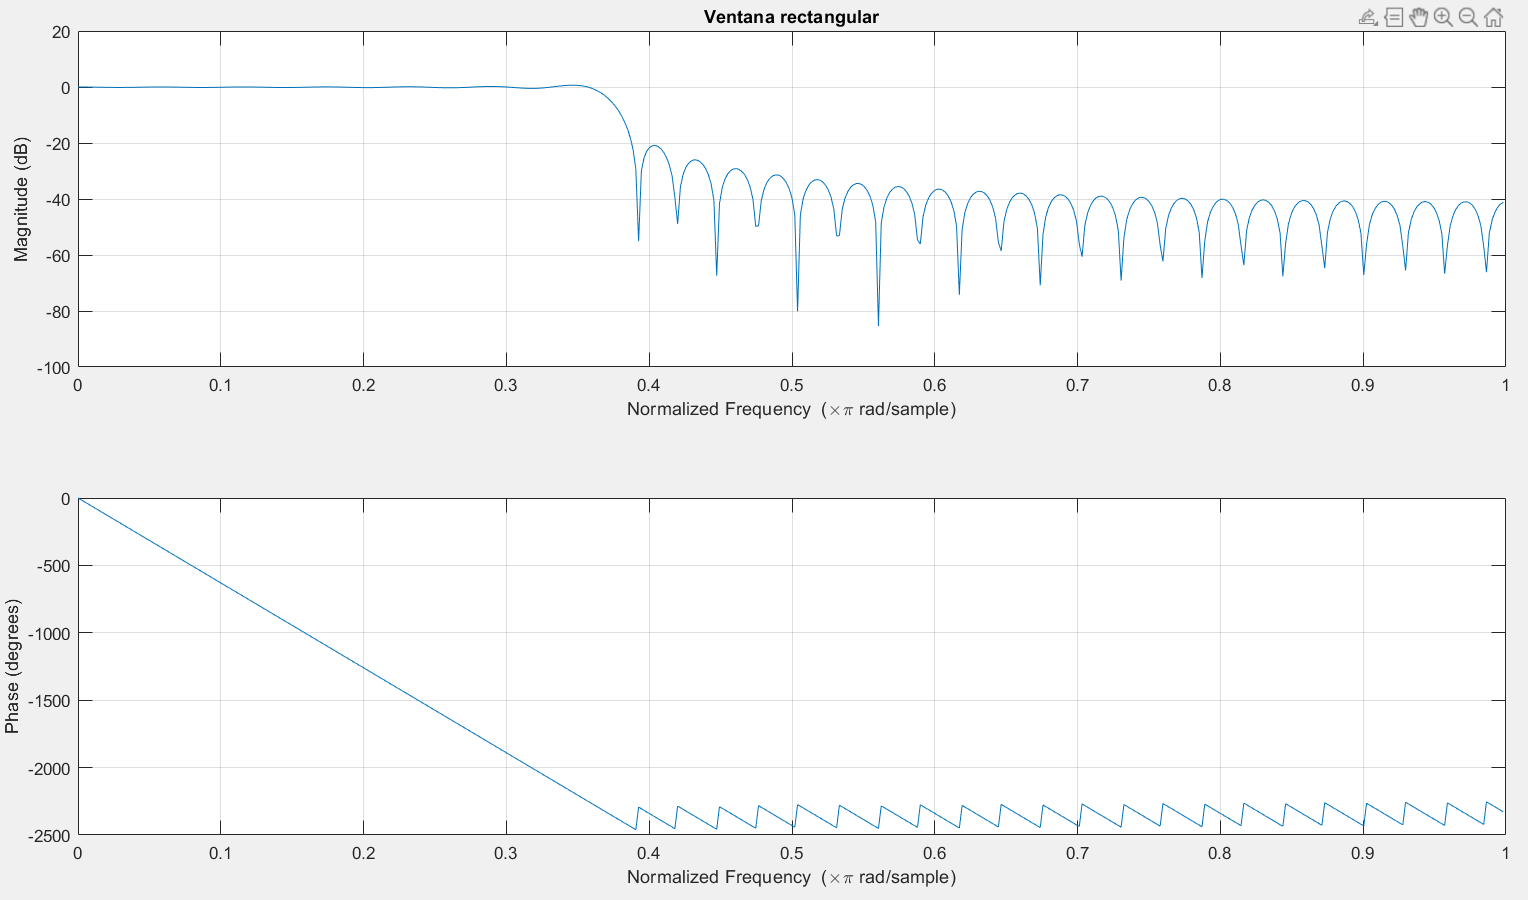
\includegraphics[width=0.75 \linewidth]{Figuras/III_1)rect2.png}
        \caption{Magnitud y fase del filtro con ventana cuadrada.}
        \label{fig:III_1)cuadrada}
    \end{figure}
    \begin{figure}[H]
        \centering
        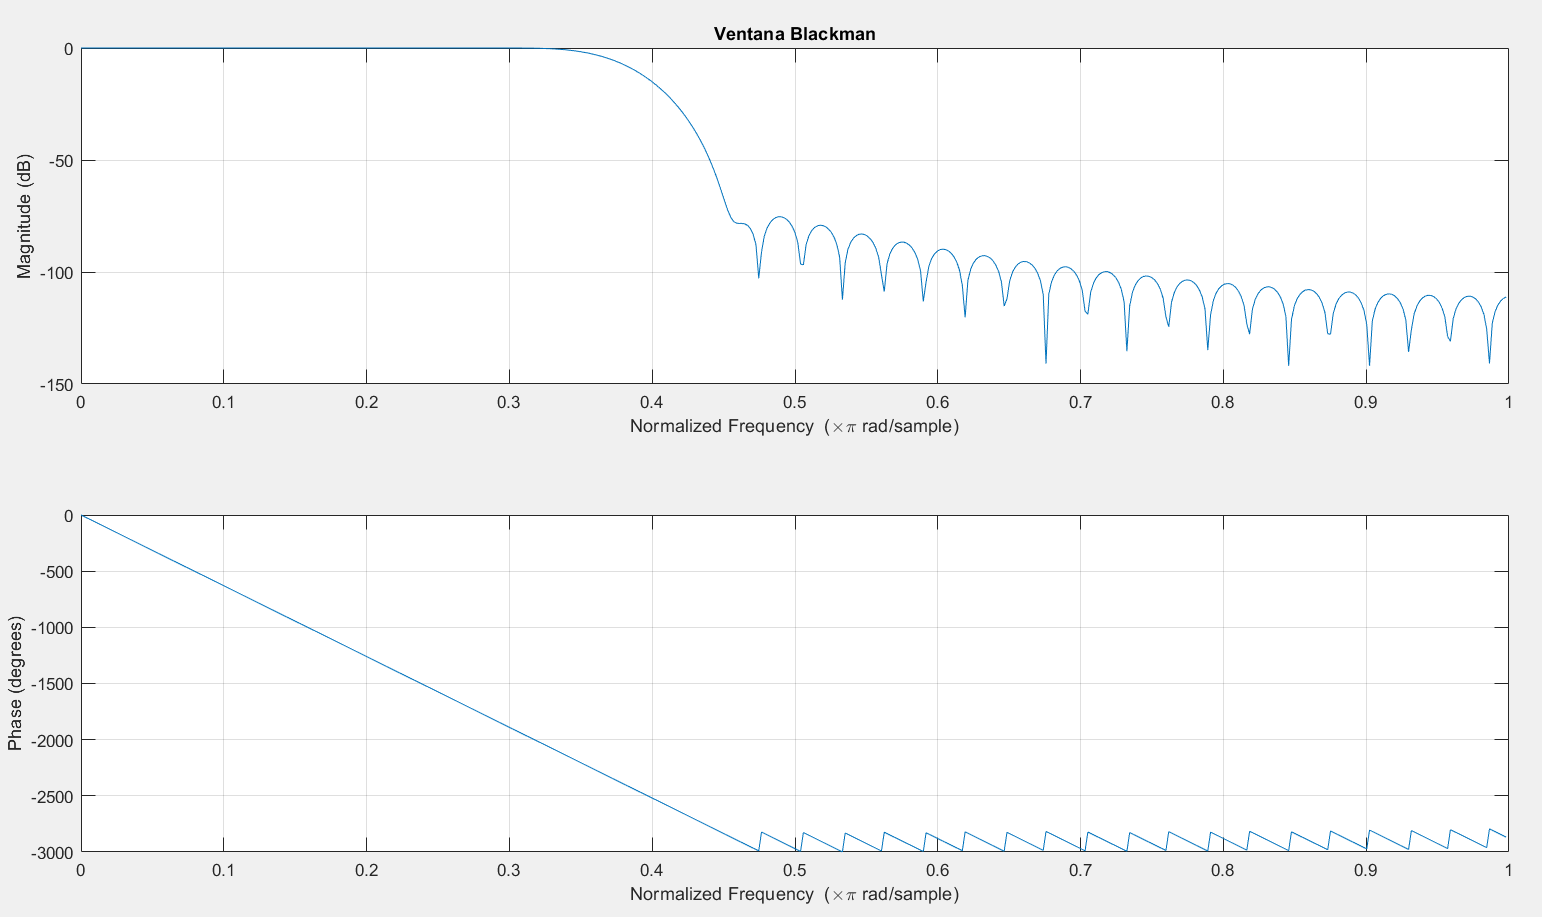
\includegraphics[width=0.75 \linewidth]{Figuras/III_1)blackman2.png}
        \caption{Magnitud y fase del filtro con ventana blackman.}
        \label{fig:III_1)blackman}
    \end{figure}
    \item%2)-------------------------------------------------------------------------%
    Las respuestas en magnitud para valores de N iguales a 70 y 150 se encuentran en las Figuras \ref{fig:III_2)70} y \ref{fig:III_2)150} respectivamente.
    
    Se aprecia que al aumentar el orden del filtro la atenuación de la banda de rechazo es mayor, en este caso de unos 10 dB, además, el paso a la banda de rechazo es más abrupta. Teniendo esto en cuenta, si la aplicación deseada es muy exigente se podría considerar el filtro de mayor orden por la mejora en la banda de transición.  
    
    Por lo tanto se genera una mayor atenuación en las zonas de rechazo, además de una zona de transición entre banda de paso y de rechazo más corta.
    \begin{figure}[H]
        \centering
        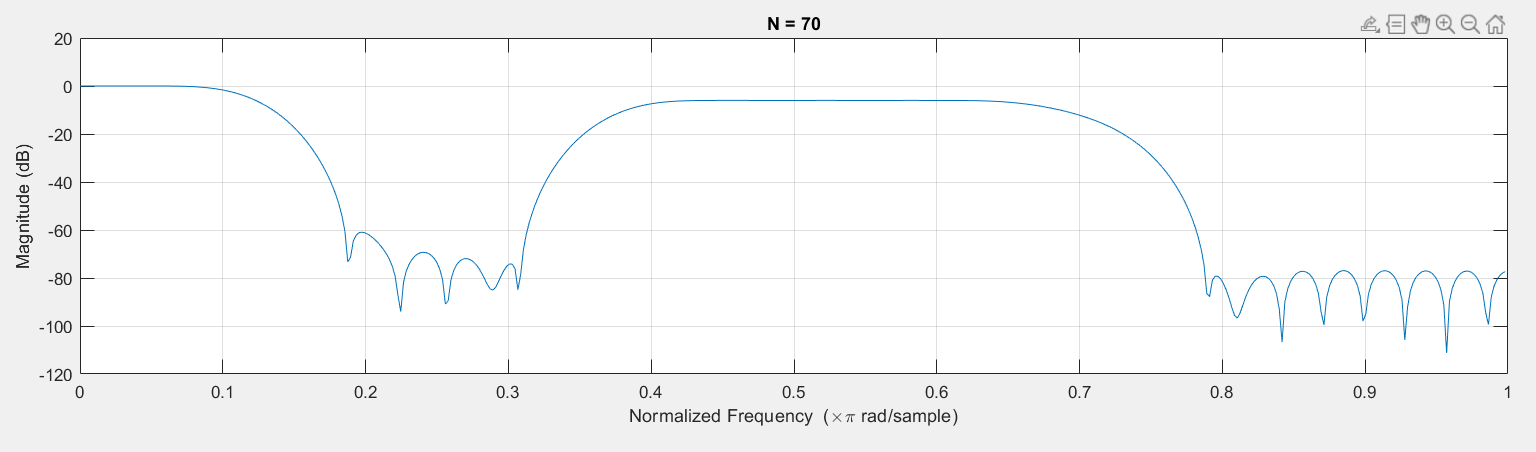
\includegraphics[width=0.75 \linewidth]{Figuras/III)_2)70.png}
        \caption{Magnitud del filtro de orden 70.}
        \label{fig:III_2)70}
    \end{figure}
    \begin{figure}[H]
        \centering
        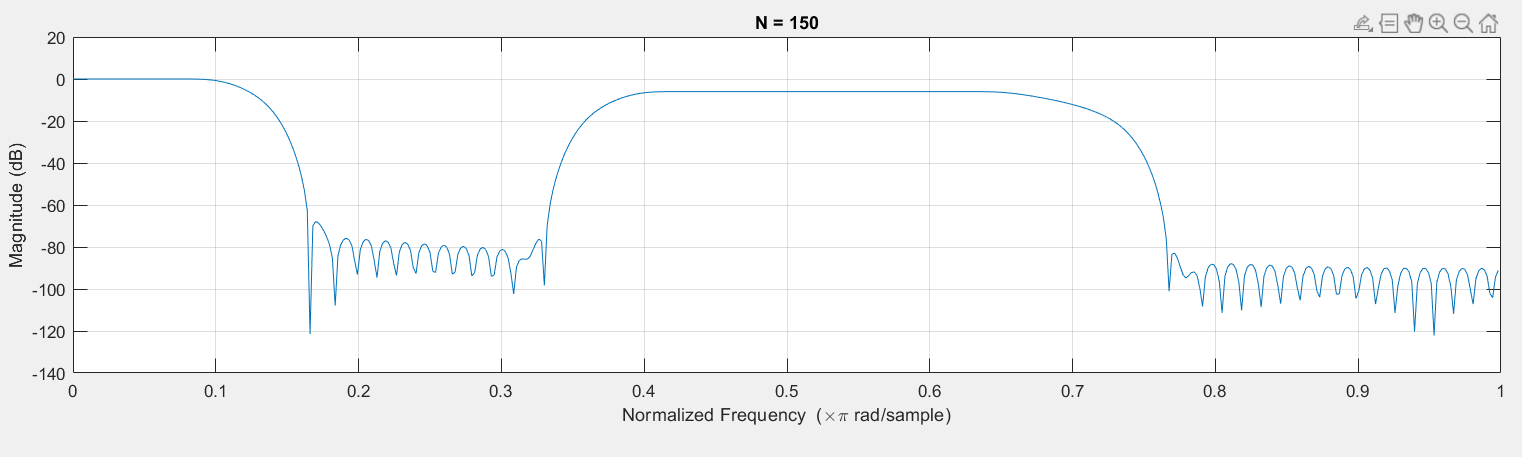
\includegraphics[width=0.75 \linewidth]{Figuras/III_2)150.png}
        \caption{Magnitud del filtro de orden 150.}
        \label{fig:III_2)150}
    \end{figure}
    
    
    \item%3)-------------------------------------------------------------------------%
    El comando \texttit{firpm}, es un algorítmo que diseña un filtro según el algoritmo de Parks-McClellan. Este entrega los coeficientes del filtro óptimo, recibiendo como entradas el orden del filtro, y la respuesta en frecuencia deseada (siendo esta ingresada mediante un vector de frecuenias normalizadas y un vector de amplitudes para cada frecuencia).
    
    La función tiene la forma \texttt{b = firpm(n,f,a)}, donde b son los coeficientes del filtro, n el orden del filtro, f el vector de frecuencias y a el vector de amplitudes requeridas para cada frecuencia.
    
    Estos valores pueden ser obtenidos desde el comando \textit{firpmord}, el cual entrega el orden del filtro requerido a partir de condiciones como las frecuencias de paso y de corte y el ripple de banda de paso y de rechazo. También entrega los arreglos f y a para obtener el filtro óptimo a partir de \textit{firpm}.
    
    
\end{enumerate}

%%%%%%%%%%%%%%%%%%%%%%%%%%%%%%%%%%%%%%%%%%%%%%%%%%%%%%%%%%%%%%%%%%%%%%%%%%%%%%%%%
%
%---------DISE ̃NO DE FILTROS IIRMEDIANTE HERRAMIENTAS DEMATLAB-----------------%
%
%%%%%%%%%%%%%%%%%%%%%%%%%%%%%%%%%%%%%%%%%%%%%%%%%%%%%%%%%%%%%%%%%%%%%%%%%%%%%%%%%
\section{Diseño de filtros IIR usando herramientas de Matlab}
\begin{enumerate}[1)]
    \item%1)-------------------------------------------------------------------------%
Siguiendo las recomendaciones de $help~ellip$ usamos los parámetros $Rp = 0.5$
y $Rs = 20$, donde $Rp$ es el máximo rizado en la banda de paso y $Rs$ es la atenuación mínima en la banda de paso, por lo que tendremos un máximo 
$ripple$ de $0.5~dB$ en las bandadas de paso y una atenuación mínima de $20~dB$ en las bandas de rechazo. Esto se cumple en todos los filtros diseñados a continuación. \\
        \begin{enumerate}[a)]
            \item %a)-------------------------------------------------------------------------%
            
                Para el filtro pasa-bajos el resultado se muestra en la Figura \ref{fig:IV_1a}.
                \begin{figure}[H]
                \centering
                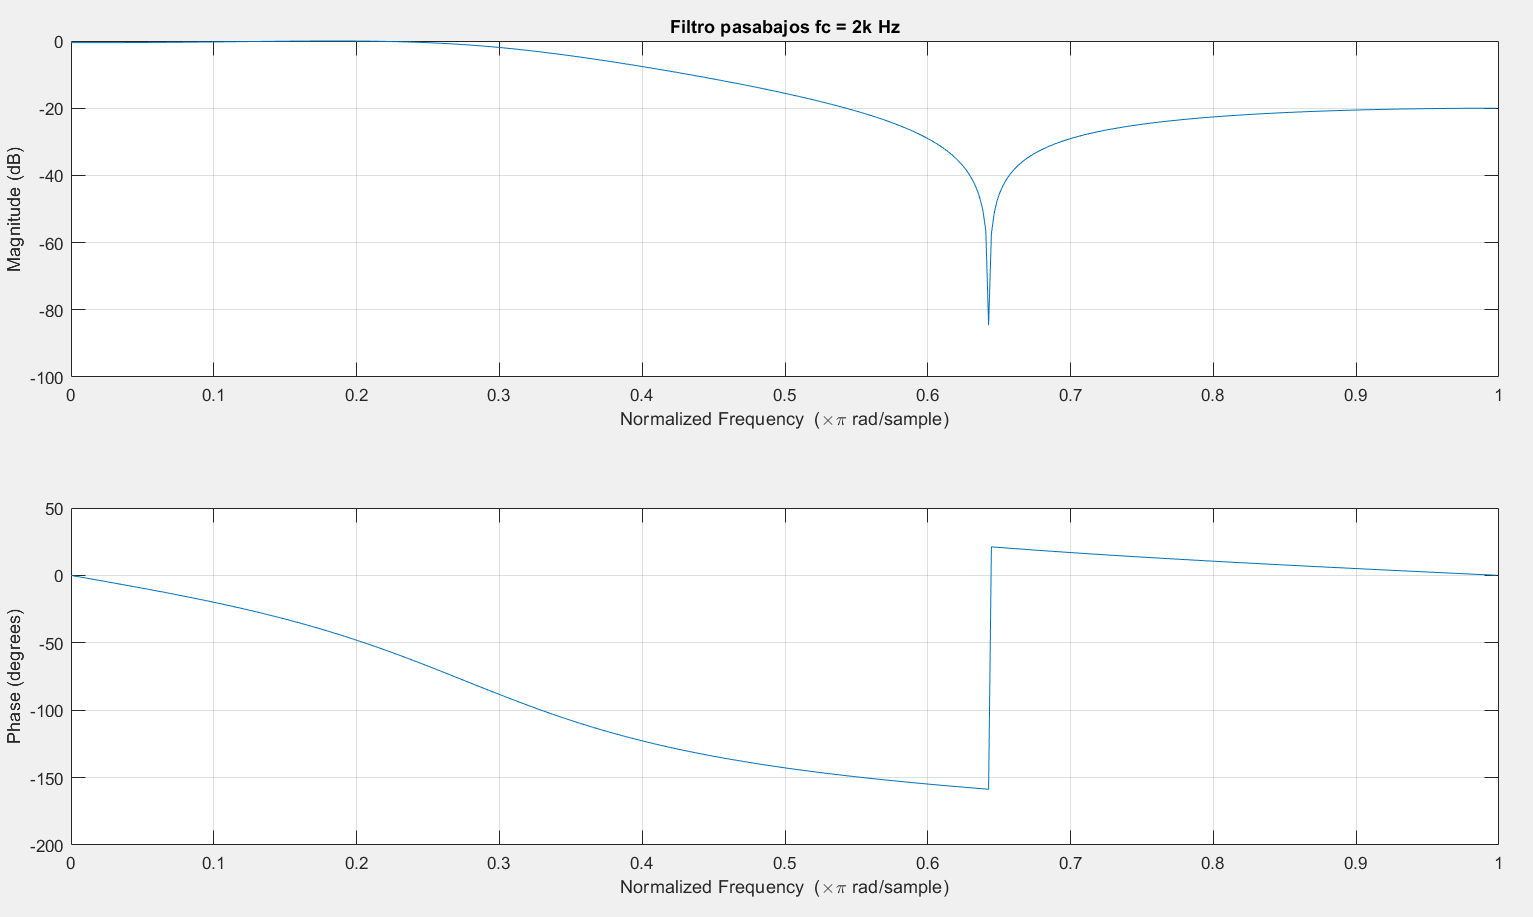
\includegraphics[width=0.75 \linewidth]{Figuras/IV_1)a).png}
                \caption{Magnitud y fase del filtro pasa-bajos de orden 2.}
                \label{fig:IV_1a}
                 \end{figure}
             
            \item %b)-------------------------------------------------------------------------%
            
                Para el filtro pasa-altos el resultado se muestra en la Figura \ref{fig:IV_1b}.
                \begin{figure}[H]
                \centering
                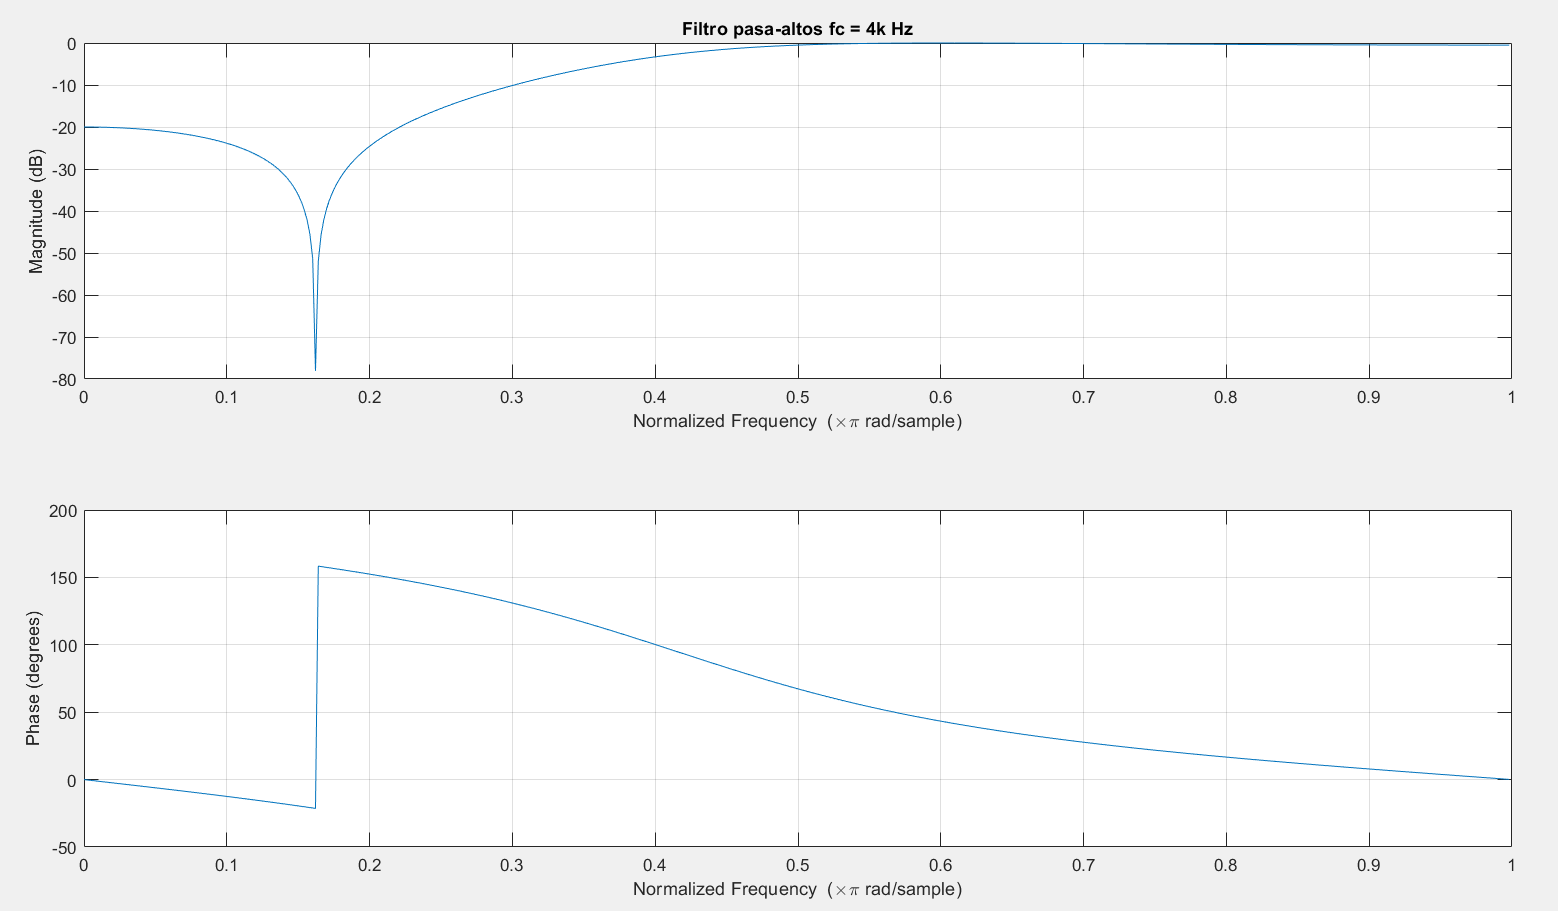
\includegraphics[width=0.75 \linewidth]{Figuras/IV_1)b).png}
                \caption{Magnitud y fase del filtro pasa-altos de orden 2.}
                \label{fig:IV_1b}
                \end{figure}
            
            \item %c)-------------------------------------------------------------------------%
            
                Para el filtro pasa-bandas el resultado se muestra en la Figura \ref{fig:IV_1c}.
                \begin{figure}[H]
                \centering
                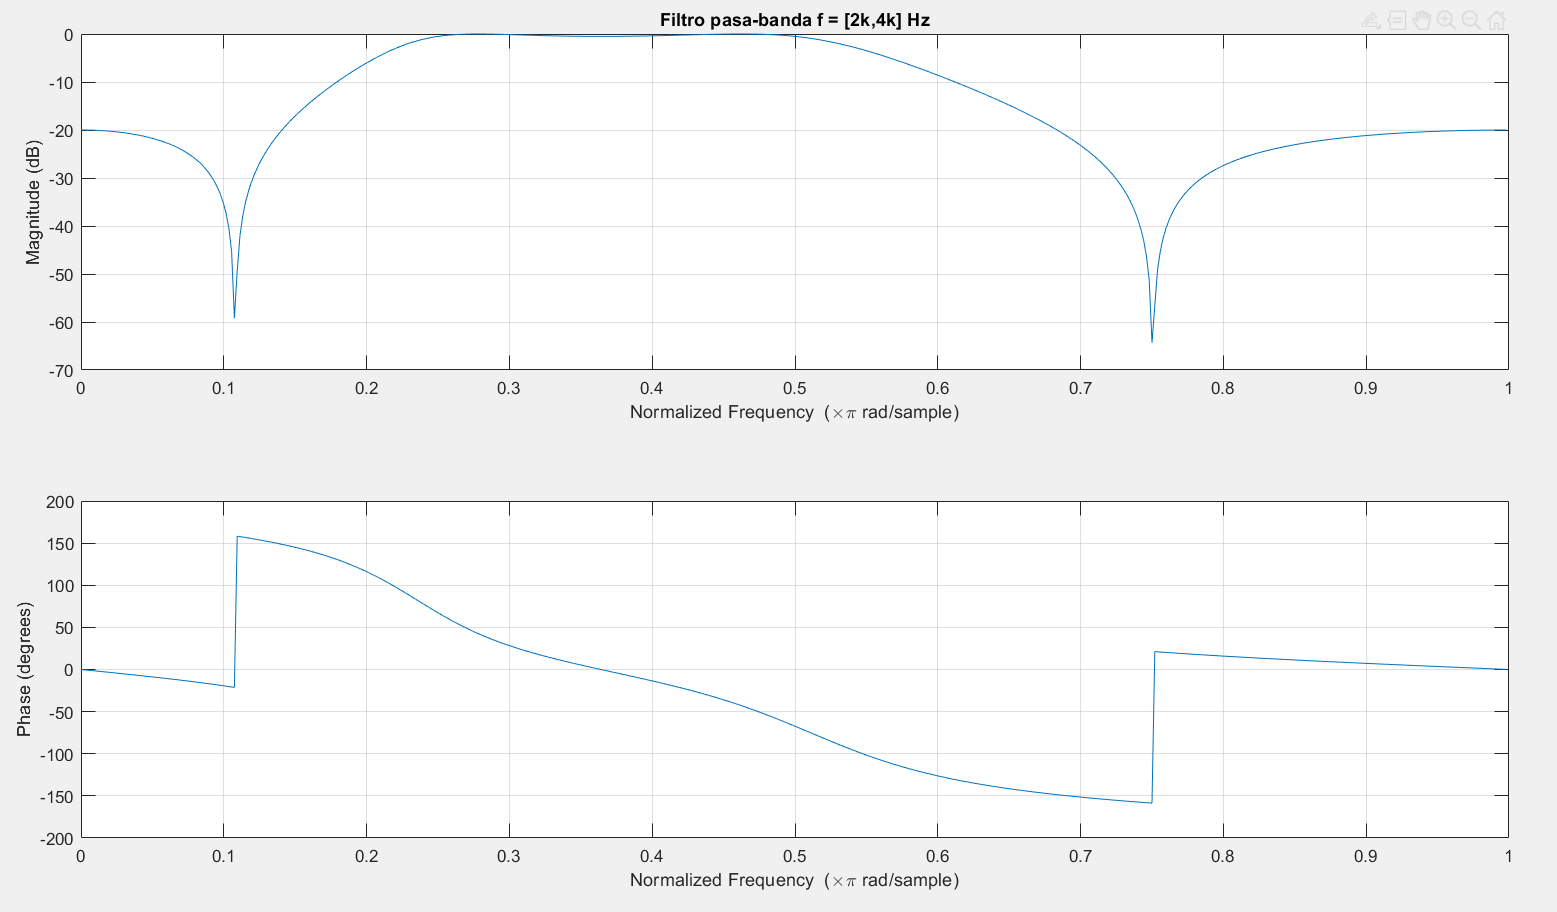
\includegraphics[width=0.75 \linewidth]{Figuras/IV_1)c).png}
                \caption{Magnitud y fase del filtro pasa-bandas de orden 4.}
                \label{fig:IV_1c}
                \end{figure}
                
            \item %d)-------------------------------------------------------------------------%
            
                Para el filtro elimina-bandas el resultado se muestra en la Figura \ref{fig:IV_1d}.
                \begin{figure}[H]
                \centering
                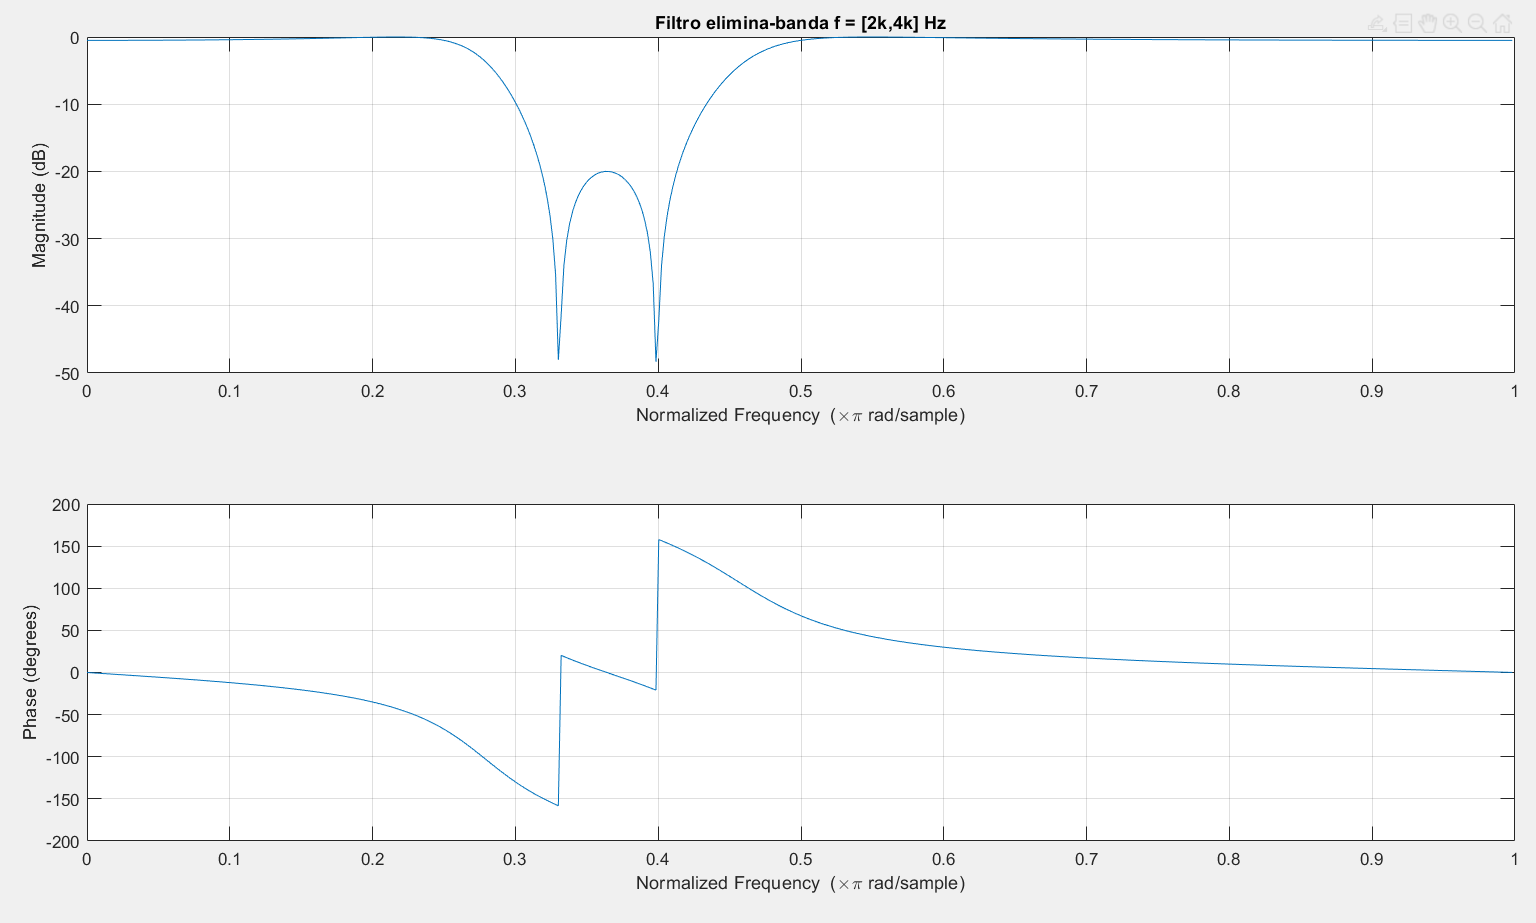
\includegraphics[width=0.75 \linewidth]{Figuras/IV_1)d).png}
                \caption{Magnitud y fase del filtro elimina-bandas de orden 4.}
                \label{fig:IV_1d}
                \end{figure}
                
        \end{enumerate}
    
    \item %2)-------------------------------------------------------------------------%
        El comando \textit{Cheby1} obtiene los coeficientes de función de transferencia de un filtro Chebyshev especificando la frecuencia de borde de banda de paso y el ripple de la banda de paso, mientras que el comando \textit{Cheby2} lo hace especificando la frecuencia de borde de banda de rechazo y la atenuación de banda de rechazo.
        \begin{enumerate}[a)]
            \item %a)-------------------------------------------------------------------------%
                Elegimos el comando $Cheby1$ ya que este nos permite configurar el nivel peak-to-peak en decibelios del rizado en la banda de paso, en este caso $R=2$. El resultado se muestra en la Figura \ref{fig:IV_2a}. \\
                
                \begin{figure}[H]
                \centering
                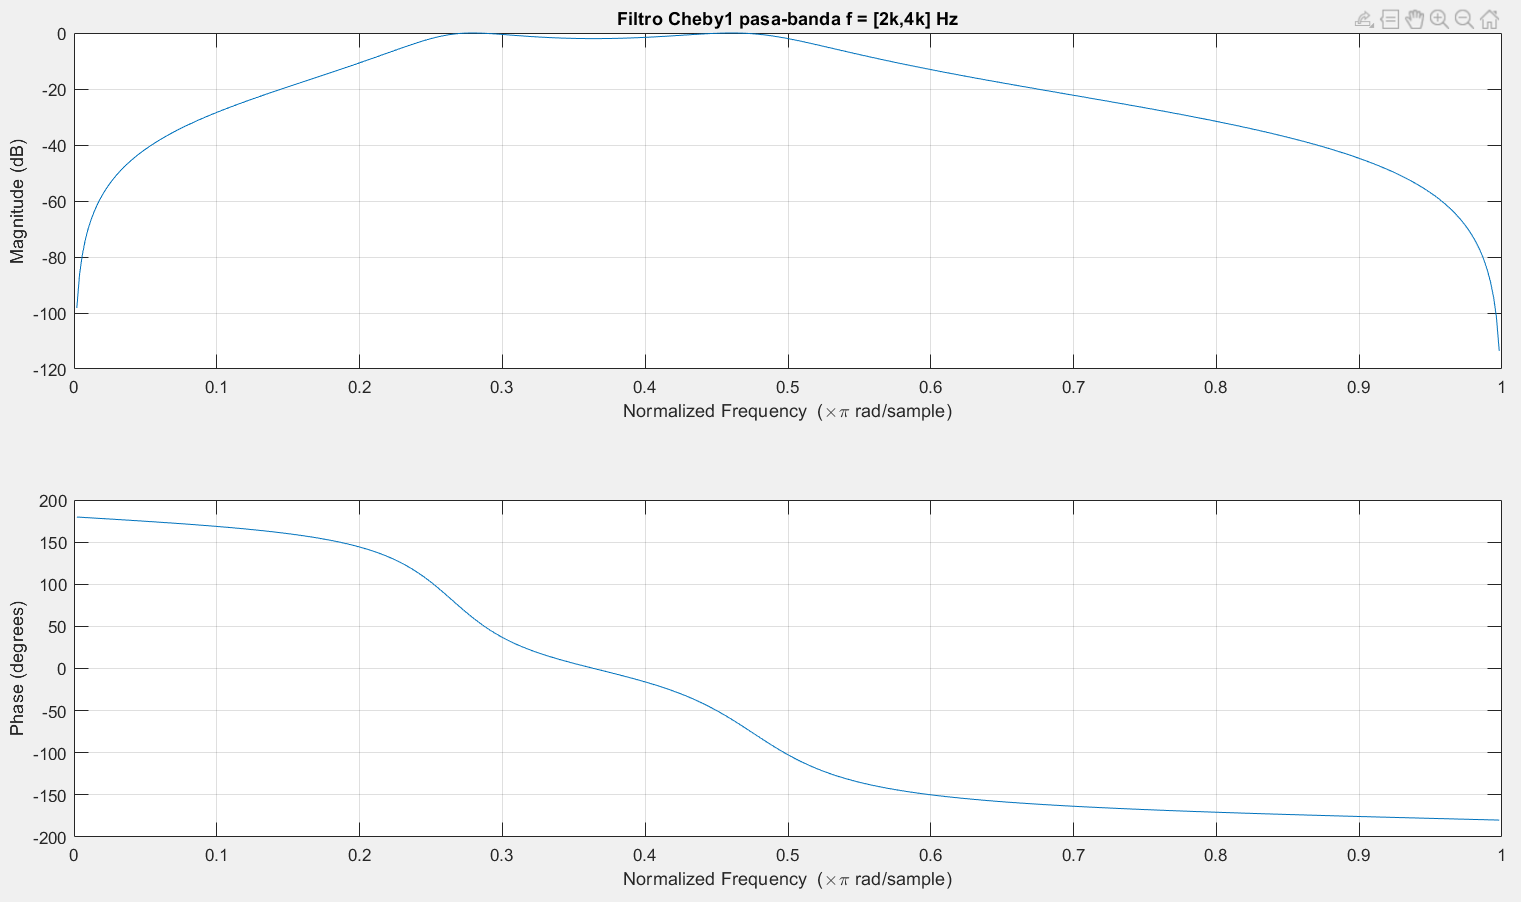
\includegraphics[width=0.75 \linewidth]{Figuras/IV_2)a).png}
                \caption{Magnitud y fase del filtro pasa-bandas de orden 4 para Chevy1.}
                \label{fig:IV_2a}
                \end{figure}
                
            \item %b)-------------------------------------------------------------------------%
                Elegimos el comando $Cheby2$ ya que nos permite configurar la mínima atenuación en decibelios en la banda de rechazo, en este caso $R=20$. El resultado se muestra en la Figura \ref{fig:IV_2b}.
                
                \begin{figure}[H]
                \centering
                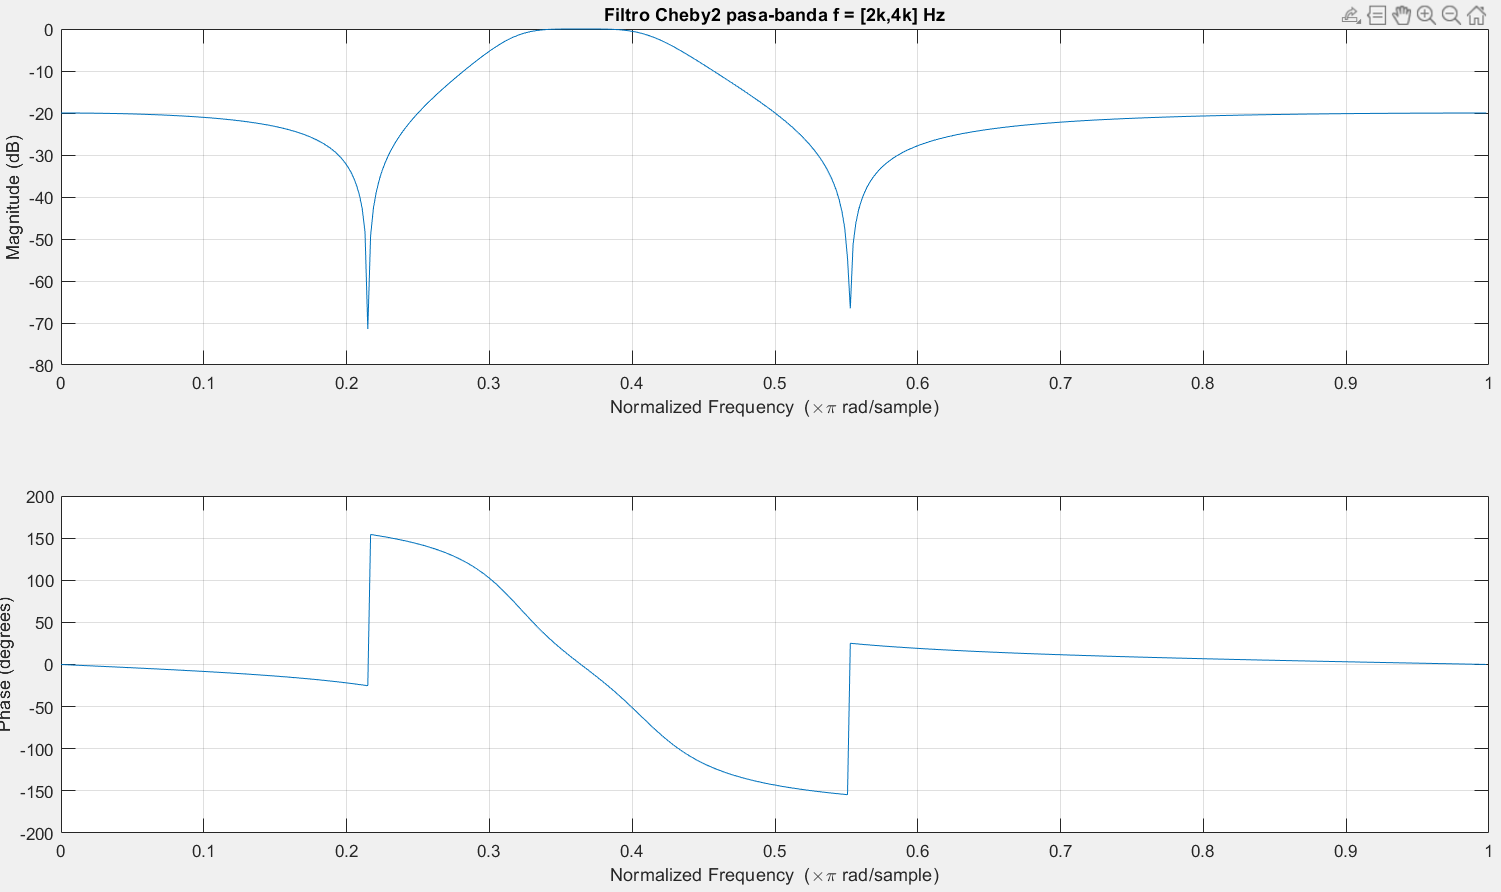
\includegraphics[width=0.75 \linewidth]{Figuras/IV_2)b).png}
                \caption{Magnitud y fase del filtro pasa-bandas de orden 4 para Chevy2.}
                \label{fig:IV_2b}
                \end{figure}
                
        \end{enumerate}
    
    \item %3)-------------------------------------------------------------------------%
    
        El resultado del la respuesta en frecuencia del filtro Butterworth se muestra en la Figura \ref{fig:IV_3}.
        \begin{figure}[H]
        \centering
        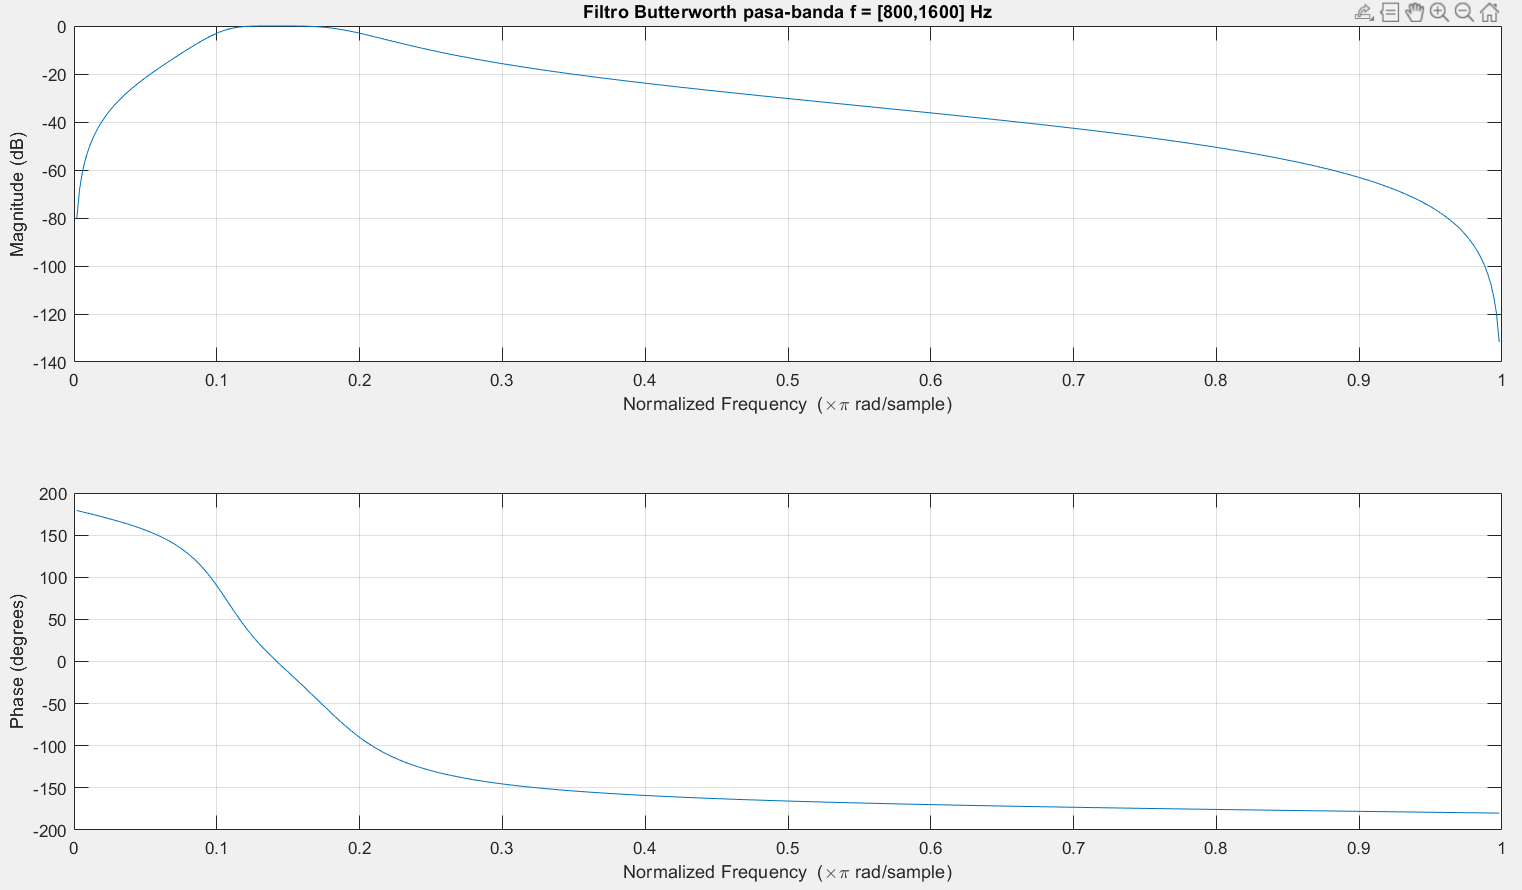
\includegraphics[width=0.75 \linewidth]{Figuras/IV_3).png}
        \caption{Magnitud y fase del filtro Butterworth pasa-bandas de orden 4.}
        \label{fig:IV_3}
        \end{figure}
        
        Notamos que al aumentar en N el orden del filtro Butterworth, aumentan en N tanto los polos como los ceros del sistema.\\
        Para el filtro Butterworth de orden 4, tenemos 2 pares de polos conjugados y 4 ceros, de forma similar para el filtro de orden 8, tenemos 4 pares de polos conjugados y 8 ceros. Esto se muestra en las Figuras \ref{fig:IV_3)1} y \ref{fig:IV_3)2} para los ordenes 4 y 8 respectivamente.
        
                \begin{figure}[H]
                \centering
                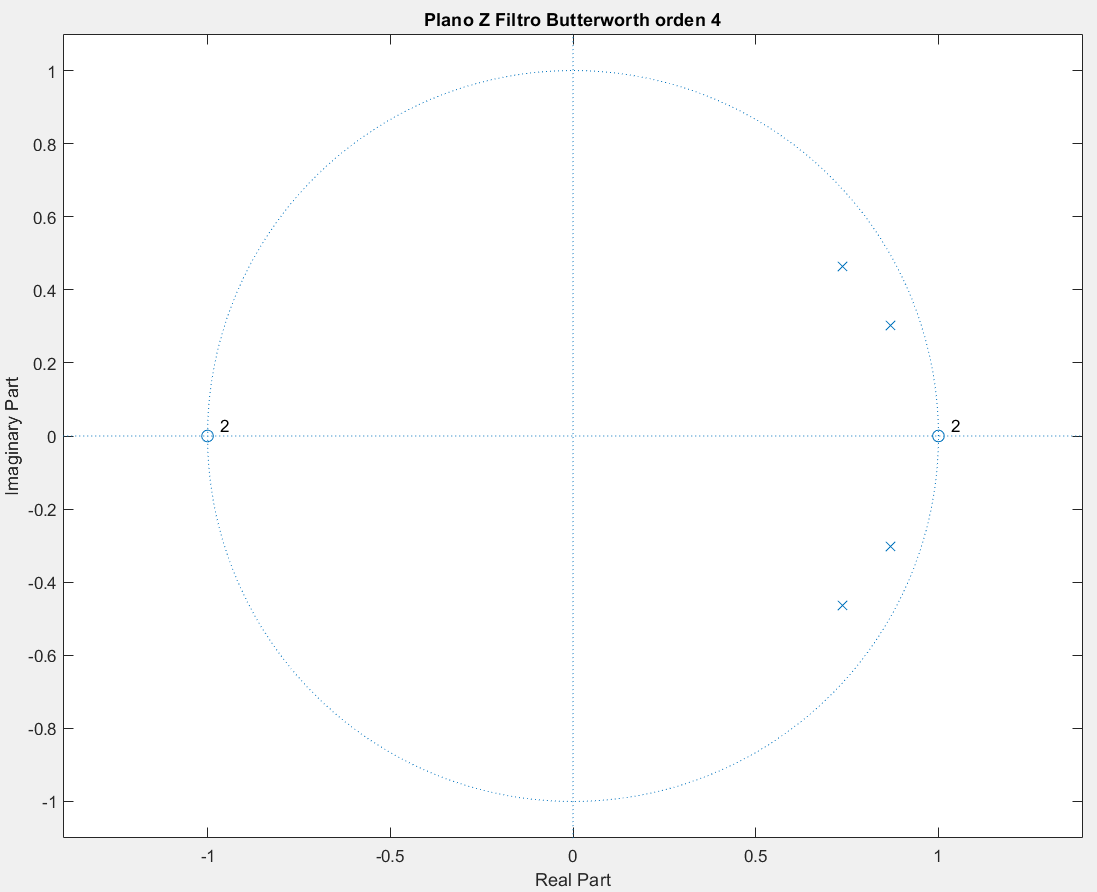
\includegraphics[width=0.75 \linewidth]{Figuras/IV_3)1.png}
                \caption{Plano Z de Filtro Butterworth orden 4}
                \label{fig:IV_3)1}
                \end{figure}
                
                \begin{figure}[H]
                \centering
                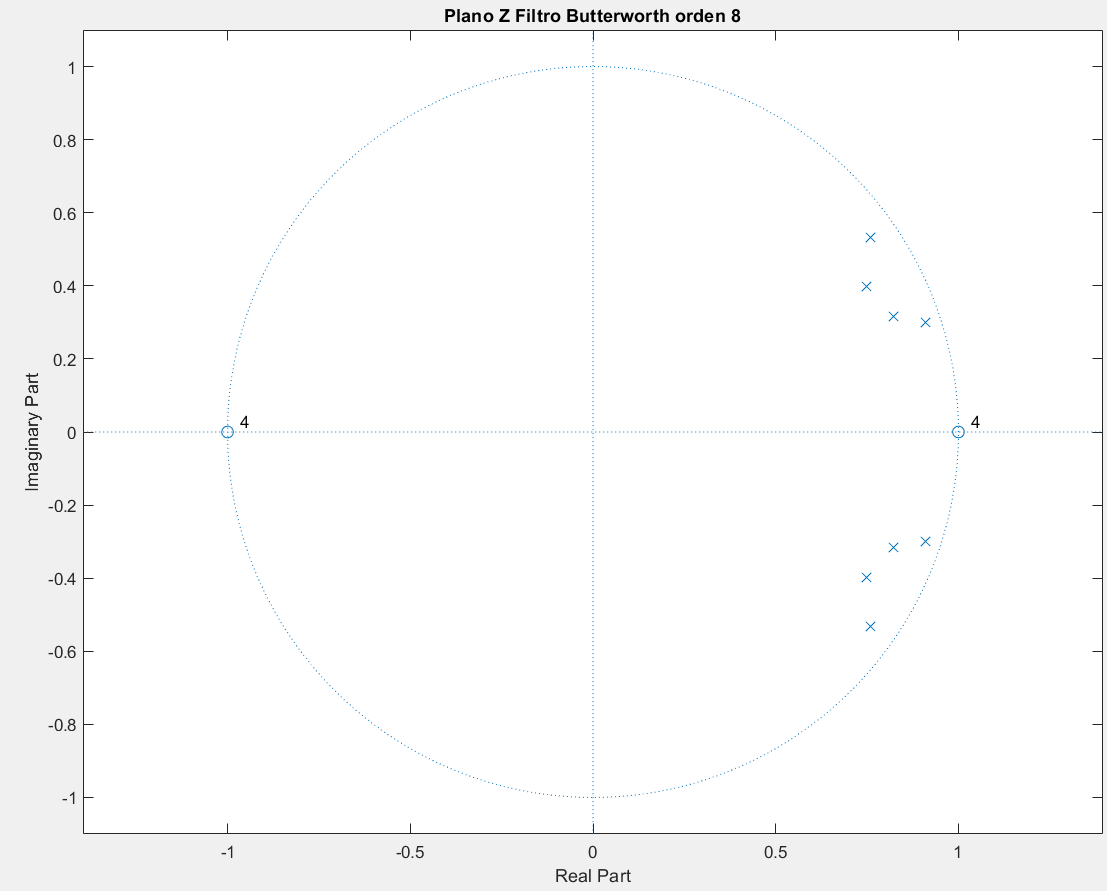
\includegraphics[width=0.75 \linewidth]{Figuras/IV_3)2.png}
                \caption{Plano Z de Filtro Butterworth orden 8}
                \label{fig:IV_3)2}
                \end{figure}
        
\end{enumerate}

%%%%%%%%%%%%%%%%%%%%%%%%%%%%%%%%%%%%%%%%%%%%%%%%%%%%%%%%%%%%%%%%%%%%%%%%%%%%%%%%%
%
%---COMPARACI ́ON DE DISE ̃NOS ́OPTIMOS DE FILTROSFIREIIR------------------------%
%
%%%%%%%%%%%%%%%%%%%%%%%%%%%%%%%%%%%%%%%%%%%%%%%%%%%%%%%%%%%%%%%%%%%%%%%%%%%%%%%%%
\section{Comparación de diseños óptimos de filtros FIR e IIR}
\begin{enumerate}[1)]
    \item %1)-------------------------------------------------------------------------%
    Se calculó el orden de los filtros Butterworth, Chebyshev, Elliptic y FIR equiripple para que cumplan los requisitos requeridos.
    
    Para esto se utilizó el siguiente código.
    \begin{lstlisting}
    fp = 2400;
    fsp = 4000;
    fs = 16000;
    Rp = 0.5; %decibeles
    Rs = 40; %decibeles 
    
    [n_butter,wn_butter] = buttord(fp/fs,fsp/fs,Rp,Rs);
    [n_cheb,wn_cheb] = cheb1ord(fp/fs,fsp/fs,Rp,Rs);
    [n_ellip,wn_ellip] = ellipord(fp/fs,fsp/fs,Rp,Rs);
    
    f = [fp fsp];
    a = [1 0];
    dev = [(10^(Rp/20)-1)/(10^(Rp/20)+1)  10^(-Rs/20)];
    
    [n_fir,fo_fir,ao_fir,w_fir] = firpmord(f,a,dev,fs);
    \end{lstlisting}
    
    La tabla de comparación se muestra a continuación:
\begin{table}[H]
        \centering
        \begin{tabular}{|c|c|c|}
        \hline
            Filtro     & Orden & Tipo \\ \hline
            Butterworth & 11 & IIR \\
            Chebyshev     & 6 & IIR \\
            Elliptic     & 4 & IIR \\
            Equiripple    & 16 & FIR \\\hline
        \end{tabular}
        \caption{Orden requerido para que los filtros cumplan los requisitos.}
        \label{tab:1}
\end{table}

Se comprueba que los filtro FIR requieren orden mayor que los filtros IIR para cumplir los mismos requisitos.
        
\end{enumerate}
%%%%%%%%%%%%%%%%%%%%%%%%%%%%%%%%%%%%%%%%%%%%%%%%%%%%%%%%%%%%%%%%%%%%%%%%%%%%%%%%%
%
%--IMPLEMENTACI ́ON EN S-FUNCTIONS: FILTROBIQUAD---------R------------------------%
%
%%%%%%%%%%%%%%%%%%%%%%%%%%%%%%%%%%%%%%%%%%%%%%%%%%%%%%%%%%%%%%%%%%%%%%%%%%%%%%%%%
\section{Implementación en s-function: filtro Biquad}
\begin{enumerate}[1)]
    \item %1)-------------------------------------------------------------------------%
        
        Se creó la función \texttt{float filterBiquad(bqState\_t *filterNState, float filterInput)} la cual filtra la señal de entrada según un filtro bicuadrático cuyos parámetros se determinan en la estructura \texttt{bqState\_t}.

        El código de la función es el siguiente:
        \begin{lstlisting}[language=C]
        static double filterBiquad(bqState_t *filterNState, double filterInput)
{
    filterNState->bqInput[2]=filterNState->bqInput[1];
    filterNState->bqInput[1]=filterNState->bqInput[0];
    filterNState->bqInput[0]=filterInput;
    filterNState->bqOutput[2]=filterNState->bqOutput[1];
    filterNState->bqOutput[1]=filterNState->bqOutput[0];
    filterNState->bqOutput[0]=((filterNState->bqB0*filterNState->bqInput[0]+
    filterNState->bqB1*filterNState->bqInput[1]
            +filterNState->bqB2*filterNState->bqInput[2])-(filterNState->bqA1*filterNState->bqOutput[1]
            +filterNState->bqA2*filterNState->bqOutput[2]));
            
    return filterNState->bqOutput[0];
}
\end{lstlisting}
Al experimentar alimentando el sistema con un delta de Kronecker, se observa que se generan oscilaciones levemente mayores al aumentar el ancho de banda.

Por otro lado, al probar la función en la señal \texttt{alternate\_tones.wav}, se observa que al disminuír el ancho de banda, la respuesta transitoria entre la señal filtrada y la parte nula de la señal, es mayor.

Las figuras \ref{fig:VI-1a} y \ref{fig:VI-1b} muestran los resultados del filtrado de la señal \texttt{alternate\_tones.wav} para un ancho de banda de $50$ y de $200~Hz$. Corroborando el correcto filtrado del tono correspondiente a $400~Hz$, y observando la diferencia en las respuestas transiente previamente mencionadas. 
\begin{figure}[H]
    \centering
    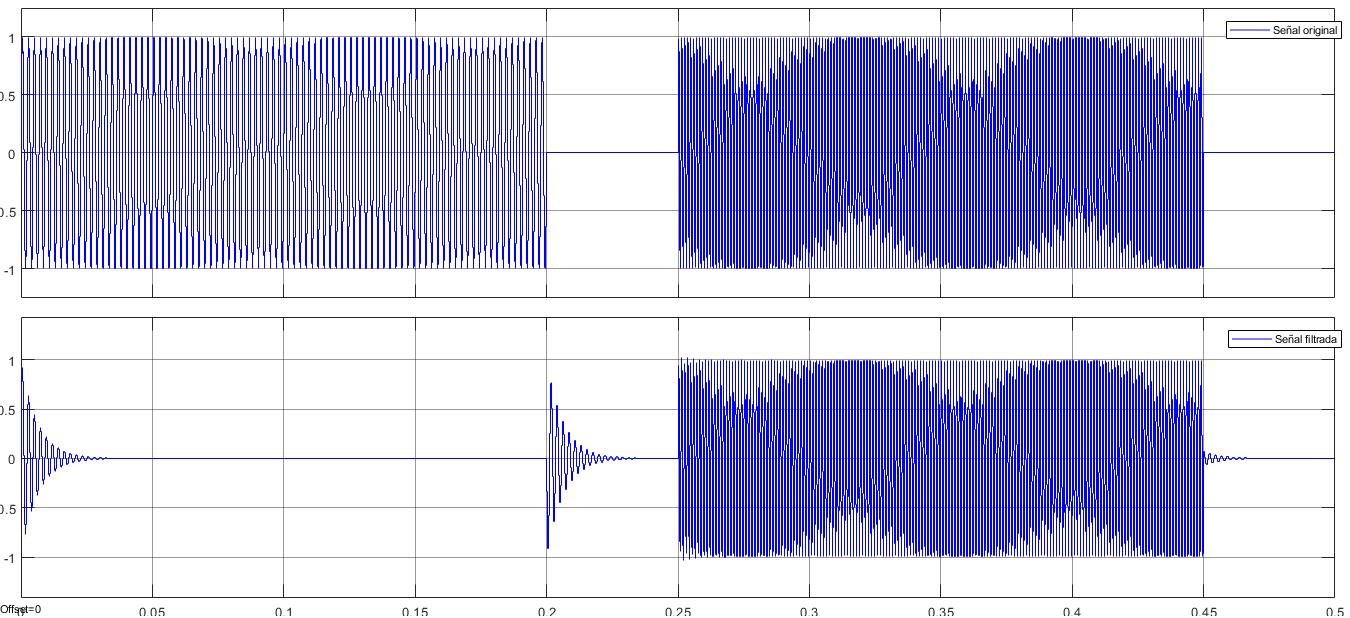
\includegraphics[width = 0.7 \linewidth]{Figuras/VI-1_BW50.png}
    \caption{Señal original y señal filtrada para frecuencia central $440~Hz$ y ancho de banda de $50~Hz$}
    \label{fig:VI-1a}
\end{figure}
\begin{figure}[H]
    \centering
    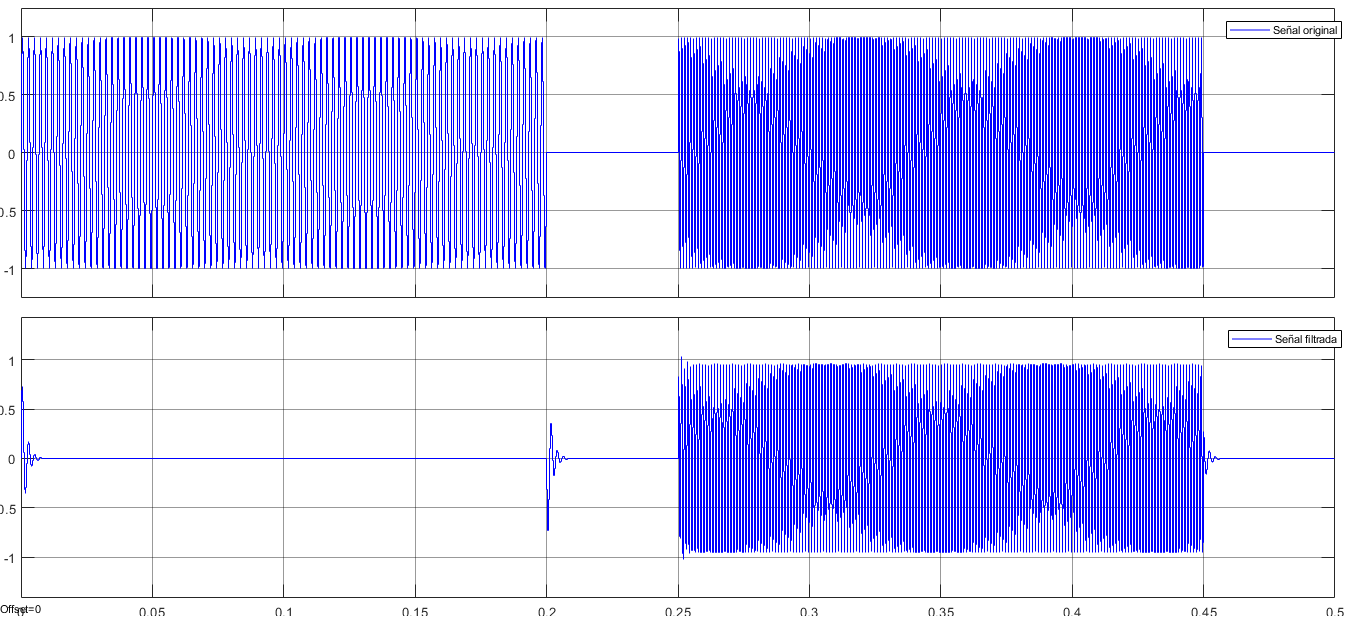
\includegraphics[width = 0.7 \linewidth]{Figuras/VI-1_BW200.png}
    \caption{Señal original y señal filtrada para frecuencia central $440~Hz$ y ancho de banda de $200~Hz$}
    \label{fig:VI-1b}
\end{figure}
    
    \item %2)-------------------------------------------------------------------------%
    Se creó la siguiente función que calcula la respuesta de un filtro Notch en relación a una frecuencia sintonizable mediante otra entrada a la \texttt{s-Function}.
    \begin{lstlisting}[language=C]
    void filterInterface(double data, double frec, double *output1)
{
    int BW = 200;
    int fs = 16000;
    
    double theta = 2*3.1415169265358979323846*frec/fs;
    double bw = 2*3.1415169265358979323846*BW/fs;
    double d = (1-sin(bw))/cos(bw);
    double gain = (1+d)/2;
    static bqState_t filtro_notch = {
        0,
        0,
        0,
        0,
        0,
        {0,0,0},
        {0,0,0}
    };
    filtro_notch.bqA1=-(1+d)*cos(theta);
    filtro_notch.bqA2=d;
    filtro_notch.bqB0=gain;
    filtro_notch.bqB1=-2*cos(theta)*gain;
    filtro_notch.bqB2=gain;
    
    *output1 = filterBiquad(&filtro_notch, data);
}
    \end{lstlisting}
    La figura \ref{fig:VI2} muestra los resultados obtenidos al aplicar está funcion utilizando como segunda entrada una frecuencia variable obtenida a partir del bloque \textit{Repeating Sequence Interpolated}. Donde se observa como pasa de eliminar el primer tono hasta eliminar el segundo tono. 
    \begin{figure}[H]
        \centering
        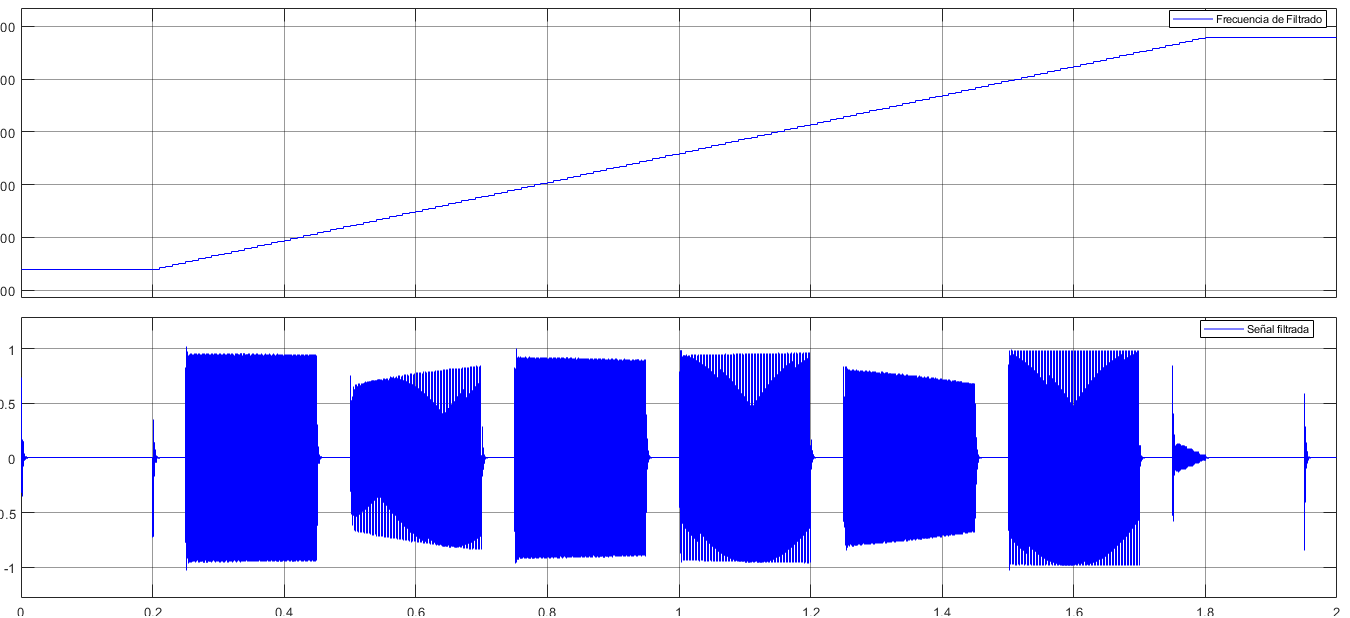
\includegraphics[width=0.7 \linewidth]{Figuras/VI-2.png}
        \caption{Señal filtrada mediante frecuencia ajustable}
        \label{fig:VI2}
    \end{figure}
    Se generó un archivo de audio con el filtrado lineal de frecuencias, donde se puede observar la transición entre escuchar solo el tono de $440~Hz$, escuchar ambos y escuchar el de $880~Hz$. El archivo ha sifo incluido bajo el nombre \texttt{filtered\_alternate\_tones.wav}.
    \item %3)-------------------------------------------------------------------------%
    Se completaron las funciones requeridas dentro del archivo \texttt{dtmf.c} de tal forma que la señal de entrada entre a $7$ filtros pasabanda diferentes, y la salida de cada uno de estos filtros entra como vector a la función \texttt{dtmfDetection}.
    
    Como las frecuencias de interés mas cercanas entre si están separadas por $73[Hz]$, y el filtro a usar es solamente de orden 2, se necesita usar un ancho de banda considerablemente menor a $73[Hz]$. En este caso se utilizarán $15[Hz]$ para cada filtro. 
    
    Se ingresó la entrada a 7 filtros diferentes con la misma estructura (pero distintos parámetros) y luego el arreglo resultante a la función de deteccion, de la siguiente manera:
    \begin{lstlisting}[language=C]
    tonesInputs[0] = bandpass_filter(input1,&filtro0,697);
    tonesInputs[1] = bandpass_filter(input1,&filtro1,770);
    tonesInputs[2] = bandpass_filter(input1,&filtro2,852);
    tonesInputs[3] = bandpass_filter(input1,&filtro3,941);
    tonesInputs[4] = bandpass_filter(input1,&filtro4,1209);
    tonesInputs[5] = bandpass_filter(input1,&filtro5,1336);
    tonesInputs[6] = bandpass_filter(input1,&filtro6,1477);
    
    *output1 = dtmfDetection(tonesInputs);
    \end{lstlisting}
    Donde la función de filtraje es la siguiente:
    \begin{lstlisting}[language=C]
    double bandpass_filter(double data, bqState_t *filterNState, int frec)
{
    int BW = 15;
    int fs = 16000;
    
    double theta = 2*3.14159265358979323846*frec/fs;
    double bw = 2*3.14159265358979323846*BW/fs;
    double d = (1-sin(bw))/cos(bw);
    double gain = (1-d)/2;
    filterNState->bqA1=-(1+d)*cos(theta);
    filterNState->bqA2=d;
    filterNState->bqB0=gain;
    filterNState->bqB1=0;
    filterNState->bqB2=-gain;

    return filterBiquad(filterNState, data);
    \end{lstlisting}
    
    La señal obtenida luego del filtraje se puede observar en la figura \ref{fig:VI-3}. Donde se obtiene que la secuencia ingresada corresponde a $\#031415926535897*$.
    
    \begin{figure}[H]
        \centering
        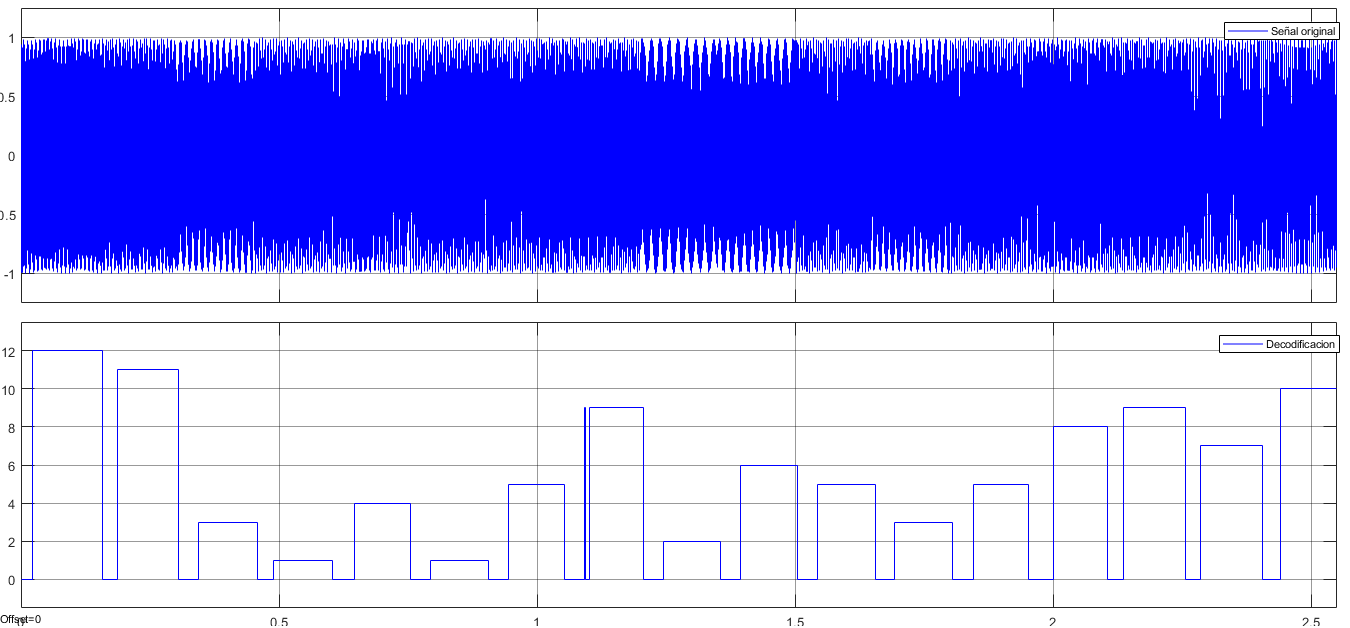
\includegraphics[width=0.8 \linewidth]{Figuras/VI-3.png}
        \caption{Secuencia DTMF original y decodificación obtenida por la s-Function}
        \label{fig:VI-3}
    \end{figure}
    
    Las carácterísticas para cada filtro se observan en la siguiente tabla, en cada caso se utilizó un filtro pasa banda bicuadrático en el cual los parámetros fueron obtenidos directamente de la frecuencia central y el ancho de banda.
    \begin{table}[H]
        \centering
        $$
        \begin{array}{|c|c|c|c|c|c|c|c|}
        \hline
        &f_0 & BW &b_0 &b_1 &b_2 &a_1 & a_2 \\
        \hline
        Filtro_0& 697~Hz & 15~Hz & 0.0029 & 0 & -0.0029 & -1.9199 & 0.9941 \\
        Filtro_1& 770~Hz & 15~Hz & 0.0029 & 0 & -0.0029 & -1.9037 & 0.9941 \\
        Filtro_2& 852~Hz & 15~Hz & 0.0029 & 0 & -0.0029 & -1.8835 & 0.9941 \\
        Filtro_3& 941~Hz & 15~Hz & 0.0029 & 0 & -0.0029 & -1.8595 & 0.9941 \\
        Filtro_4& 1209~Hz & 15~Hz & 0.0029 & 0 & -0.0029 & -1.7736 & 0.9941 \\
        Filtro_5& 1336~Hz & 15~Hz & 0.0029 & 0 & -0.0029 & -1.7259 & 0.9941 \\
        Filtro_6& 1477~Hz & 15~Hz & 0.0029 & 0 & -0.0029 & -1.6680 & 0.9941 \\
        \hline
        \end{array}
        $$
        \caption{Características de filtros aplicados. }
        \label{tab:my_label}
    \end{table}
\end{enumerate}
\end{document}
